% -*- root: main.tex -*-

\chapter{Unstable Cooperations}\label{UnstableCooperationsChapter}


In \Cref{StableContextLecture} (and more broadly in \Cref{ChapterFiniteSpectra}), we codified the structure of the stable $E$--cooperations acting on the $E$--homology of a spectrum $X$, attached to it the $E$--Adams spectral sequence which approximates the stable homotopy groups $\pi_* X$, and gave algebro-geometric descriptions of the stable cooperations for some typical spectra: $\HFtwo$, $MO$, and $MU$.  We will now pursue a variation on this theme, where we consider the $E$--homology of a \emph{space} rather than of a generic spectrum.  In this Case Study, we will examine the theory of cooperations that arises from this set-up, called the \textit{unstable $E$--cooperations}.  This broader collection of cooperations has considerably more intricate structure than their stable counterparts, requiring the introduction of a new notion of an unstable context.  With that established, we will again find that $E$--homology assigns spaces to quasicoherent Cartesian sheaves over the unstable context, and we will again assemble an \emph{unstable} $E$--Adams spectral sequence approximating the \emph{unstable} homotopy groups of the input space, whose $E^2$--page in favorable situations is tracked by the cohomology of the sheaf over the unstable context.

Remarkably, these unstable contexts also admit algebro-geometric interpretations.  In finding the right language for this, we introduce different subclasses of cooperations (e.g., \textit{additive}), and we are also naturally led to consider \textit{mixed cooperations} (as we did stably in \Cref{OrientationsOnEAndMU}) of the form $F_* \OS{E}{*}$.  The running theme is that when $E$ and $F$ are complex-orientable, there is a natural approximation map \[\Spec Q^* F_* \OS{E}{*} \to \InternalHom{FormalGroups}(\CP^\infty_F, \CP^\infty_E)\] which is an isomorphism in every situation of interest.  However, these isomorphisms do not appear to admit uniform proofs\footnote{The best uniform result I can find is due to Butowiez and Turner~\cite[Theorem 3.12]{ButowiezTurner}.}, so we instead investigate the following cases by hand:
\begin{itemize}
\item (\Cref{UnstableContextsSection}:) For $F = E = \HFtwo$, we compute the full unstable dual Steenrod algebra $\HFtwo_* \OS{\HFtwo}{*}$ by means of iterated bar spectral sequences.  We then pass to the additive unstable cooperations, where we show by hand that this presents the endomorphism scheme $\InternalHom{FormalGroups}(\G_a, \G_a)$.  Finally, we pass to the stable additive cooperations, and we check that our results here are compatible with the isomorphism \[\Spec \HFtwo_* \HFtwo \cong \InternalAut{\G_a}\] presented in \Cref{SteenrodAlgIdentifiedWithAutGa}.
\item (\Cref{COableCoopnsII}:) We next consider the case where $E = MU$ and where $F$ is any complex-orientable theory.  We begin with the case $F = \HFp$, where we can again approach the problem using iterated bar spectral sequences.  The resulting computation is sufficiently nice that we can use this special case of $F = \HFp$ to deduce the further case of $F = H\Z_{(p)}$, then $F = H\Z$, then $F = MU$, and then finally $F$ any complex-orientable theory.
\item (\Cref{LEFTCooperations}:) Having been able to vary $F$ as widely as possible in the previous case, we then turn to trying to vary $E$.  This is considerably harder, since the infinite loopspaces $\OS{E}{*}$ associated to $E$ are extremely complicated and vary wildly under even ``small'' changes in $E$.  However, in the special case of $F = \HFp$, we have an incredibly powerful trick available to us: Dieudonn\'e theory, discussed in \Cref{SectionDieudonneModules}, gives an equivalence of categories \[D_*\co \CatOf{GradedHopfAlgebras}^{> 0, \fin}_{\F_p/} \to \CatOf{GradedDMods},\] and applying this in the composite
\begin{align*}
\CatOf{Spectra} & \xrightarrow{\Loops^\infty} \CatOf{Loopspaces} \\
& \xrightarrow{\HFp_*} \CatOf{GradedHopfAlgebras}^{>0, \fin}_{\F_p/} \\
& \xrightarrow{D_*} \CatOf{GradedDMods} \\
& \subseteq \CatOf{GradedModules}_{\Cart}
\end{align*}
gives a homological functor.  This means that the Dieudonn\'e module associated to an infinite loopspace varies stably with the spectrum underlying the loopspace, which is enough leverage to the settle the case where $E$ is any Landweber--flat theory.
\item (\Cref{CoopnsForMoravaKandHA}:) Finally, we settle one further case not covered by any of our generic hypotheses above: $F = K_\Gamma$ and $E = H\Z/p^j$.  Neither $K_\Gamma$ nor $H\Z/p^j$ is Landweber--flat, but because $K_\Gamma$ is a field spectrum and because the additive group law associated to $H\Z/p^j$ is so simple, we can still perform the requisite iterated bar spectral sequence calculation by hand.
\end{itemize}

This last case is actually our real goal, as we are about to return to the project outlined in the Introduction.  In the language of \Cref{IntroAHSMU6Thm}, choosing $\Gamma$ to be the formal completion of an elliptic curve at the identity section presents the spectra $K_\Gamma$ and $E_\Gamma$ of \Cref{NilpotenceAndPeriodicity} as the most basic examples of \textit{elliptic spectra}.  The goal of that Theorem is to study $E_* BU[6, \infty)$ for $E$ an elliptic spectrum, so when proving it in \Cref{ChapterSigmaOrientation} we will be led to consider the fiber sequences
\begin{align*}
B\SU \to BU & \to \OS{H\Z}{2}, & \OS{H\Z}{3} \to BU[6, \infty) & \to B\SU,
\end{align*}
which mediate the difference between $E_* BU$ and $E_* BU[6, \infty)$ by means of $E_* \OS{H\Z}{2}$ and $E_* \OS{H\Z}{3}$.  Thus, in our pursuit of $K_\Gamma{}_* BU[6, \infty)$, we will want to have $K_\Gamma{}_* \OS{H\Z}{*}$ already in hand, as well as an algebro-geometric interpretation of it.









\section{Unstable contexts and the Steenrod algebra}\label{UnstableContextsSection}

In this Lecture, our goal is to codify the study of unstable cooperations, beginning with an unstructured account of how they arise.  Recall that for a ring map $f\co R \to S$, in \Cref{StableContextLecture} we studied the problem of recovering an $R$--module from an $S$--module plus extra data.  The intermediate category of extra data that we settled on was that of \index{descent!data}\textit{descent data}, which we phrased most enduringly as a certain cosimplicial diagram.  Stripping away the commutative algebra, the only categorical formality that went into this was the adjunction
\begin{center}
\begin{tikzcd}
\CatOf{Modules}_R \arrow[shift left=0.4em]{r}{- \otimes_R S} & \CatOf{Modules}_S \arrow[shift left=0.4em, "\mathrm{forget}"]{l} ,
\end{tikzcd}
\end{center}
or later on, when given a ring spectrum $\eta\co \S \to E$, the adjunction
\begin{center}
\begin{tikzcd}
\CatOf{Spectra} = \CatOf{Modules}_{\S} \arrow[shift left=0.4em]{r}{- \sm E} & \CatOf{Modules}_E \arrow[shift left=0.4em, "\mathrm{forget}"]{l} .
\end{tikzcd}
\end{center}
The identification of $\CatOf{Modules}_S$ with $T$--algebras in $\CatOf{Modules}_R$ for the monad $T = \mathrm{forget} \circ (- \otimes_R S)$ is the objective of \index{descent!monadic}\textit{monadic descent}~\cite[Theorem 4.7.4.5]{LurieHA}.  This categorical recasting is ignorant of some of the algebraic geometry we discovered next, but it is suitable for us now as we consider the composition with a second adjunction:
\begin{center}
\begin{tikzcd}
\CatOf{Spaces} \arrow[shift left=0.4em]{r}{\Susp^\infty} & \CatOf{Spectra} = \CatOf{Modules}_{\S} \arrow[shift left=0.4em]{r}{- \sm E} \arrow[shift left=0.4em]{l}{\Loops^\infty} & \CatOf{Modules}_E \arrow[shift left=0.4em, "\mathrm{forget}"]{l} .
\end{tikzcd}
\end{center}
We will write $E(-)$ for the induced monad on $\CatOf{Spaces}$, given by the formula \[E(X) = \Loops^\infty (E \sm \Susp^\infty X) = \colim_{j \to \infty} \Loops^j (\OS{E}{j} \sm X),\] where $\OS{E}{*}$ are the constituent spaces in the $\Omega$--spectrum of $E$.  This space has the property $\pi_* E(X) = \widetilde E_{* \ge 0} X$.  The monadic structure comes from the two evident natural transformations:
\[\eta\co X \to \Loops^\infty \Susp^\infty X \simeq \Loops^\infty (\S \sm \Susp^\infty X) \to \Loops^\infty (E \sm \Susp^\infty X) = E(X),\]
\begin{align*}
\mu\co E(E(X)) & = \Loops^\infty(E \sm \Susp^\infty\Loops^\infty(E \sm \Susp^\infty X)) \\
& \to \Loops^\infty(E \sm E \sm \Susp^\infty X) \to \Loops^\infty(E \sm \Susp^\infty X) = E(X).
\end{align*}
Just as in the stable situation, we can extract from this a cosimplicial space:
\begin{definition}
The \index{descent!object!unstable}\textit{unstable descent object} is the cosimplicial space
\[\sheaf{UD}_E(X) := \left\{
\begin{tikzcd}
\begin{array}{c} E \\ \circ \\ X \end{array} \arrow[leftarrow, shift left=\baselineskip]{r}{\mu} \arrow[shift left=(2*\baselineskip)]{r}{\eta_L} \arrow{r}{\eta_R} &
\begin{array}{c} E \\ \circ \\ E \\ \circ \\ X \end{array} \arrow[shift left=(3*\baselineskip)]{r} \arrow[leftarrow, shift left=(2*\baselineskip)]{r} \arrow[shift left=\baselineskip]{r}{\Delta} \arrow[leftarrow]{r} \arrow[shift right=\baselineskip]{r} &
\begin{array}{c} E \\ \circ \\ E \\ \circ \\ E \\ \circ \\ X \end{array} \arrow[shift left=(4*\baselineskip)]{r} \arrow[leftarrow, shift left=(3*\baselineskip)]{r} \arrow[shift left=(2*\baselineskip)]{r} \arrow[leftarrow, shift left=\baselineskip]{r} \arrow{r} \arrow[leftarrow, shift right=\baselineskip]{r} \arrow[shift right=(2*\baselineskip)]{r} &
\cdots
\end{tikzcd}
\right\}.\]
Its totalization gives the \index{completion!unstable}\textit{unstable $E$--completion of $X$}.  The simplicial scheme \[\Ucontext{E} = \Spec \pi_0 \sheaf{UD}_E(S^0)\] forms the \index{context!unstable}\textit{unstable context} for $E$, and a space $X$ gives rise to a quasicoherent sheaf \[\Ucontext{E}(X) = (\pi_0 \sheaf{UD}_E(X))\widetilde{}.\]
\end{definition}

The remainder of this section will be spent trying to understand the spectral sequence associated to the coskeletal filtration of such an unstable descent object.  In the stable situation, we recognized that in favorite situations the homotopy groups of the descent object formed a cosimplicial module over a certain cosimplicial ring---or, equivalently, a sheaf over a certain simplicial scheme.  Furthermore, we found that the simplicial scheme itself had some arithmetic meaning, and that the $E_2$--page of the descent spectral sequence computed the cohomology of this sheaf.  We will find analogues of all of these results in the unstable setting, listed above in order from least to most difficult.

We would like to recognize the cosimplicial abelian group $\pi_0 \sheaf{UD}_E(X)$ as a sort of comodule.  In the stable case, this came from the smash product map $\S^0 \sm X \to X$, as well as the lax monoidality of the functor $\sheaf{D}_E(-)$.  However, to get a \index{Segal condition}Segal condition by which we could identify the higher-dimensional objects in $\pi_0 \sheaf D_E(X)$, we had to introduce the condition \index{flatness hypothesis@flatness hypothesis, \FH}{\FH}.\footnote{In particular, {\FH} caused the marked map in $E_0 X \xrightarrow{\eta_R} E_0(E \sm X) \xleftarrow{\star} E_0 E \otimes_{E_0} E_0 X$ to become invertible.}  The unstable situation has an analogous antecedent:

\begin{definition}[{\cite[Assumption 6.5]{BCM}}]
A ring spectrum $E$ is said to satisfy the \index{flatness hypothesis@flatness hypothesis, \FH!unstable@unstable, \UFH}\textbf{U}nstable \textbf{F}latness \textbf{H}ypothesis, or \UFH, if $E_* \OS{E}{k}$ is a free and even $E_*$--module for every value of $k$.\footnote{This helps us understand the following analogous zigzag: \[\pi_0 E(X) \xrightarrow{\eta_R} \pi_0 E(E(X)) \xleftarrow{\mu \circ 1} \pi_0 E(E(E(X))) \xleftarrow{\mathrm{compose}} \pi_m E(E(S^0)) \times \pi_0 E(X).\]}
\end{definition}

Under this condition, we again turn to studying the structure of $\sheaf{UD}_E(S^0)$.  If we had a Segal condition, we would expect the structure present to be determined by $\pi_0 \sheaf{UD}_E(S^0)[j]$ for $j \le 2$.  The data at $j = 0$ is largely redundant: \[\pi_0 E(S^0) = \pi_0 \OS{E}{0} = E_0\] computes the coefficient ring of $E$.  The data at $j = 1$ consists of the homology groups of the the infinite loopspace associated to $E$: \[\pi_0 E(E(S^0)) = E_0 \OS{E}{0}.\]  There are three pieces of structure present here: the augmentation map \[E_0 \OS{E}{0} \to E_0(E) \to E_0\] and the left- and right-unit maps $E_0 \to E_0 \OS{E}{0}$.  The assumption {\UFH} gives us a foothold on the case $j = 2$: a choice of basis for $E_0 \OS{E}{0}$ gives an unstable isomorphism $E(E(S^0)) \simeq \prod_\ell \OS{E}{0}$, so that $\pi_0 \sheaf{UD}_E(S^0)[2]$ splits as a tensor product of terms of the form $E_0 \OS{E}{0}$.  Here, we find a lot of structure: the addition of cohomology classes induces a map \[\ast\co E_0 \OS{E}{0} \otimes_{E_0} E_0 \OS{E}{0} \to E_0 \OS{E}{0};\] the multiplication induces a map \[\circ\co E_0 \OS{E}{0} \otimes E_0 \OS{E}{0} \to E_0 \OS{E}{0};\] these are compatible with the images of unit classes $0, 1 \in \pi_0 E$ under the left- and right-units specified above; there is an additive inverse map \[\chi\co E_0 \OS{E}{0} \to E_0 \OS{E}{0}\] compatible with the $\ast$--product and giving a skew-commutativity formula \[a \circ b = \chi(b \circ a);\] there is a diagonal map \[\Delta\co E_0 \OS{E}{0} \to E_0 \OS{E}{0} \otimes_{E_0} E_0 \OS{E}{0};\] each $E_0 \OS{E}{0}$ becomes a Hopf algebra using $\chi$, $\ast$, and $\Delta$; and there is a distributivity condition pictured in \Cref{DistributivityDiagram} intertwining $\ast$, $\circ$, and $\Delta$.\footnote{Analogous structure also appears for aperiodic ring spectra $E$ satisfying a graded version of {\UFH}, and in that case tracking through the extra grading indices is actually helpful for deciphering what these maps ``feel'' like.}\footnote{There are a few more pieces of structure that Boardman--Johnson--Wilson call an \textit{enriched Hopf ring}, which we omit from the definition because they do not affect the homological algebra of modules for a Hopf ring:
\begin{itemize}
\item An element $v \in \pi_0 E$ selects a connected component of $\OS{E}{0}$, and there is an attached element $[v] \in E_0 \OS{E}{0}$.
\item A cohomology operation $r\co E^0(-) \to E^0(-)$ induces a map $\OS{E}{0} \to \OS{E}{0}$ and hence a map on $E$--homology $r_*\co E_0 \OS{E}{0} \to E_0 \OS{E}{0}$.
\item In particular, this gives a homology suspension element $e = (e_2)_*$, where $e_2\co E^0(-) \to E^2(-) \cong E^0(\Susp^{-2} -)$ is the map witnessing the $2$--periodicity of $E$.
\end{itemize}}

\begin{figure}
\begin{center}
\begin{tikzcd}
A \otimes_R (A \otimes_R A) \arrow{r}{1 \otimes \ast} \arrow{d}{\Delta \otimes (1 \otimes 1)} & A \otimes_R A \arrow{dddd}{\circ} \\
\left(A \otimes_R A \right) \otimes_{R_*} (A \otimes_R A) \arrow{d}{\simeq} \\
\left(A \otimes_R A \otimes_R A \otimes_R A \right) \arrow{d}{1 \otimes \tau \otimes 1} \\
\left(A \otimes_R A \otimes_R A \otimes_R A \right) \arrow{d}{\circ \otimes \circ} \\
\left(A \otimes_R A\right) \arrow{r}{\ast} & A.
\end{tikzcd}
\end{center}
\caption{The distributivity axiom for $\ast$ over $\circ$ in a Hopf ring.}\label{DistributivityDiagram}
\end{figure}

\begin{definition}[{\cite[Summary 10.46]{BJW}}]
A \idxentry{Hopf ring} is a module along with structure maps $+$, $-$, $\cdot$, $\ast$, $\circ$, $\Delta$, and $\chi$ subject to the axioms declared above.  A Hopf ring becomes an \index{Hopf ring!enriched}\textit{enriched Hopf ring} when it is furthermore equippped with a right-unit, an augmentation, and maps \[E_0 \OS{E}{0} \times (E_0 \OS{E}{0})^\vee \to E_0 \OS{E}{0}\] (determined by composition with the dual cohomology classes in the examples of interest).
\end{definition}

\begin{lemma}\label{HopfRingFromOneRingSpectrum}
If $X$ is a space with $E_* X$ a free $E_*$--module, then $E_0 X$ furthermore forms a \index{comodule!coalgebra}coalgebra for the comonad $G$ associated to the enriched Hopf ring $\pi_0 \sheaf{UD}_E(S^0)$.
\end{lemma}
\begin{proof}
The proof is a matter of elucidating the last condition.  For $X$ satisfying this freeness condition, there is again a splitting $E(X) \simeq \prod_\ell \OS{E}{n_\ell}$.  We interpret this at the level of algebra by defining a functor \[G\co \CatOf{Modules}_{E_0}^{\mathrm{free}} \to \CatOf{Modules}_{E_0}\] which sends $E_0$ to $E_0 \OS{E}{0}$ and which splits over direct sums.  The enriched Hopf ring structure of $\pi_0 \sheaf{UD}_E(S^0)[\le 2]$ endows $G$ with a comonad structure, and the structure maps of $\pi_0 \sheaf{UD}_E(X)[\le 2]$ endow $E_0 X$ itself with the structure of a $G$--coalgebra.
\end{proof}

\begin{theorem}[{\cite[Theorem 6.17]{BCM}}]
$\pi_0 \sheaf{UD}_E(X)$ is the bar resolution for the free Hopf module comonad, and the $E_2$--page of the \index{Adams spectral sequence!unstable}unstable descent spectral sequence is presented as
\[\pushQED{\qed}
E_2^{s} = L^s\CatOf{Coalgebras}_G(E_0, E_0 X). \qedhere
\popQED
\]
\end{theorem}

At this point, it is instructive to work through an example to understand the kinds of objects we have constructed.  At first appraisal, these objects appear to be so bottomlessly complicated that it must be a hopeless enterprise to actually compute even just the enriched Hopf ring associated to a spectrum $E$.  In fact, the abundance of structure maps involved gives enough footholds that this is actually often feasible, provided we have sufficiently strong stomachs.  Our example will be the aperiodic spectrum $E = \HFtwo$, and the place to start is with a very old lemma:
\begin{lemma}
If $E$ is a spectrum with $\pi_{-1} E = 0$, then $\OS{E}{1} \simeq B\OS{E}{0}$.  Consequentially, if $E$ is a connective spectrum then $\OS{E}{n} = B^n \OS{E}{0}$ for $n \ge 0$. \qed
\end{lemma}
\noindent This is useful to us because $B(-)$ comes with a natural skeletal filtration, which we can use to form a spectral sequence.
\begin{lemma}[{\cite[Proposition 3.2]{Segal}, \cite[Theorem 2.1]{RavenelWilsonKthyOfEMSpaces}}]
Let $G$ be a topological group.  There is a convergent \index{bar spectral sequence}spectral sequence of algebras of signature \[E^1_{*, j} = F_*(\Susp G)^{\sm j} \Rightarrow F_* BG.\]  In the case that $F$ has K\"unneth isomorphisms $\widetilde F_*((\Susp G)^{\sm j}) \cong \widetilde F_*(\Susp G)^{\otimes_{F_*} j}$, the $E^2$--page is identifiable as \[E^2_{*, *} \cong \Tor^{F_* G}_{*, *}(F_*, F_*)\] and the spectral sequence is one of Hopf algebras. \qed
\end{lemma}
\begin{corollary}
If $E$ is a connective spectrum and $F$ has K\"unneth isomorphisms $\widetilde F_*(\OS{E}{j} \sm \OS{E}{j}) \cong \widetilde F_* \OS{E}{j} \otimes_{F_*} \widetilde F_* \OS{E}{j}$ for all $j$, then there is a family of spectral sequences of Hopf algebras with signatures
\[
\pushQED{\qed}
E^2_{*, *} \cong \Tor^{F_* \OS{E}{j}}_{*, *}(F_*, F_*) \Rightarrow F_* \OS{E}{j+1}. \qedhere
\popQED
\]
\end{corollary}

That this spectral sequence is multiplicative for the $\ast$--product is useful enough, but the situation is actually much, much better than this:
\begin{lemma}[{\cite[Equation 1.3]{ThomasonWilson}, \cite[Theorem 2.2]{RavenelWilsonKthyOfEMSpaces}}]\label{CircProductAndDifferentials}
Denote by $E^r_{*, *}(F_* \OS{E}{j})$ the spectral sequence considered above whose $E^2$--term is constructed from $\Tor$ over $F_* \OS{E}{j}$.  There are maps \[E^r_{*, *}(F_* \OS{E}{j}) \otimes_{F_*} F_* \OS{E}{m} \to E^r_{*, *}(F_* \OS{E}{j+m})\] which agree with the map \[F_* \OS{E}{j+1} \otimes_{F_*} F_* \OS{E}{m} \xrightarrow{\circ} F_* \OS{E}{j+m+1}\] on the $E^\infty$--page and which satisfy
\[
\pushQED{\qed}
d^r(x \circ y) = (d^r x) \circ y. \qedhere
\popQED
\]
\end{lemma}
\noindent This Lemma is obscenely useful: it means that differentials can be transported \emph{between spectral sequences} for classes which can be decomposed as $\circ$--products.  This means that the bottom spectral sequence (i.e., the case $j = 0$) exerts a large amount of control over the others---and this spectral sequence often turns out to be very computable.

We now turn to concrete computations for $E = \HFtwo$ and $F = \HFtwo$.  To ground the induction, we will consider the first spectral sequence \[\Tor^{\HFtwo_*(\F_2)}_{*, *}(\F_2, \F_2) \Rightarrow \HFtwo_* B\F_2.\]  Using that $\RP^\infty$ gives a model for $B\F_2$, we use \Cref{HF2RPinftyExample} to analyze the target of this spectral sequence: as an $\F_2$--module, we have already demonstrated an isomorphism \[\HFtwo_* B\F_2 \cong \F_2\{a_j \mid j \ge 0\}.\]  Using our further computation in \Cref{RPExampleFaulty}, we can also give a presentation of the Hopf algebra structure on $\HFtwo_* B\F_2$: it is dual to the primitively-generated polynomial algebra on a single class, so forms a divided power algebra on a single class which we will denote by $a_{()}$.  In characteristic $2$, this decomposes as \[\HFtwo_* B\F_2 \cong \Gamma[a_{()}] \cong \bigotimes_{j=0}^\infty \F_2[a_{(j)}] / a_{(j)}^2,\] where we have written $a_{(j)}$ for $a_{()}^{[2^j]}$ in the divided power structure.

\begin{corollary}
This $\Tor$ spectral sequence collapses at the $E^2$--page.
\end{corollary}
\begin{proof}
As an algebra, the homology $\HFtwo_*(\F_2)$ of the discrete space $\F_2$ is presented by a group ring, which we can identify with a truncated polynomial algebra: \[\HFtwo_*(\F_2) \cong \F_2[\F_2] \cong \F_2[[1]] / ([1]^{\ast 2} - [0]) \cong \F_2[[1] - [0]] / ([1] - [0])^{\ast 2}.\]  The $\Tor$--algebra of this is then divided power on a single class: \[\Tor^{\HFtwo_*(\F_2)}_{*, *}(\F_2, \F_2) = \Gamma[a_{()}].\]  In order for the two computations to agree, there can therefore be no differentials in the spectral sequence.
\end{proof}

We now summarize the rest of the induction:
\begin{theorem}\label{UnstableSteenrodInduction}
$\HFtwo_* \OS{\HFtwo}{t}$ is the exterior $\ast$--algebra on the $t$--fold $\circ$--products of the generators $a_{(j)} \in \HFtwo_* B\F_2$.
\end{theorem}
\begin{proof}
Noting that the case $t = 0$ is what was proved above, make the inductive assumption that this is true for some fixed value of $t \ge 0$.  The $\Tor$ groups of the associated bar spectral sequence \[\Tor^{\HFtwo_* \OS{\HFtwo}{t}}_{*, *}(\F_2, \F_2) \Rightarrow \HFtwo_* \OS{\HFtwo}{t+1}\] form a divided power algebra generated by the same $t$--fold $\circ$--products.  An analogue of another Ravenel--Wilson lemma~(\cite[Lemma 9.5]{RavenelWilsonKthyOfEMSpaces}, \cite[Claim 8.16]{Wilson}) gives a congruence \[(a_{(j_1)} \circ \cdots \circ a_{(j_t)})^{[2^{j_{t+1}}]} \equiv a_{(j_1)} \circ \cdots \circ a_{(j_t)} \circ a_{(j_{t+1})} \tag{mod $\ast$--decomposables}.\]  It follows from \Cref{CircProductAndDifferentials} that the differentials vanish:
\begin{align*}
d((a_{(j_1)} \circ \cdots \circ a_{(j_t)})^{[2^{j_{t+1}}]}) & \equiv d(a_{(j_1)} \circ \cdots \circ a_{(j_t)} \circ a_{(j_{t+1})}) \tag{mod $\ast$--decomposables} \\
& = a_{(j_1)} \circ d(a_{(j_2)} \circ \cdots \circ a_{(j_{t+1})}) \tag{\Cref{CircProductAndDifferentials}} \\
& = 0. \tag{inductive hyp.}
\end{align*}
Hence, the spectral sequence collapses.  To see that there are no multiplicative extensions, note that the only potentially undetermined multiplications occur as $\ast$--squares of exterior classes.  However, the $\ast$--squaring map is induced by the topological map \[\OS{\HFtwo}{t} \xrightarrow{\cdot 2} \OS{\HFtwo}{t},\] which is already null on the level of spaces.  It follows that there are no extensions and the induction holds.
\end{proof}

\begin{corollary}
It follows that $\circ$--product induces an isomorphism
\begin{center}
\begin{tikzcd}
\HFtwo_* \OS{\HFtwo}{*} & \arrow["\simeq"']{l} \bigoplus_{t=0}^\infty (H_*(\RP^\infty; \F_2))^{\wedge t},
\end{tikzcd}
\end{center}
where $(-)^{\wedge t}$ denotes the $t$\textsuperscript{th} exterior power in the category of Hopf algebras. \qed
\end{corollary}

\begin{remark}[{\cite[Theorems 8.5 and 8.11]{Wilson}}]
The odd--primary analogue of this result appears in Wilson's book, where again the bar spectral sequences are collapsing.  The end result is \[\HFp_* \OS{\HFp}{*} \cong \frac{\bigotimes_{I, J} \F_p[e_1 \circ \alpha_I \circ \beta_J, \alpha_I \circ \beta_J]}{(e_1 \circ \alpha_I \circ \beta_J)^{\ast 2} = 0, (\alpha_I \circ \beta_J)^{\ast p} = 0, e_1 \circ e_1 = \beta_1},\] where we have defined the following elements:
\begin{itemize}
\item $e_1 \in (\HFp)_1 \OS{\HFp}{1}$ is the \index{homology suspension}homology suspension element.
\item $\alpha_{(j)} \in (\HFp)_{2p^j} \OS{\HFp}{1}$ are the analogues of the elements considered above.
\item $\beta_{(j)} \in (\HFp)_{2p^j} \CP^\infty$ are the algebra generators of the Hopf algebra dual of the ring of functions on the formal group $\CP^\infty_{\HFp}$ associated to $\HFp$ by its natural complex orientation.
\end{itemize}
In particular, the Hopf ring is \emph{free}\index{Hopf ring!free} on these Hopf algebras, subject to the single interesting relation $e_1 \circ e_1 = \beta_{(0)}$, essentially stemming from the equivalence $S^1 \sm S^1 \simeq \CP^1$.
\end{remark}

It is now instructive to try to relate this unstable computation to the stable one from \Cref{TheSteenrodAlgebraSection} (and, particularly, its algebro-geometric interpretation in \Cref{SteenrodAlgIdentifiedWithAutGa}).  Consider the situation of cohomology operations: each stable operation consists of a family of unstable operations intertwined by suspensions, each of which is additive and takes $0$ to $0$.  In terms of an element $\psi \in E^* \OS{E}{j}$, such an unstable operation takes $0$ to $0$ exactly when it lies in the augmentation ideal, and it is additive exactly when it satisfies Hopf algebra primitivity: \[\Delta^* \psi^* = (\psi \otimes \psi)^* \Delta^*.\]
\begin{definition}
In the setting of unstable homology cooperations, we define an \index{operations!unstable}\textit{additive unstable operation} to be one which lies in the \index{Hopf ring!star indecomposables@$\ast$--indecomposables}$\ast$--indecomposable quotient $Q_* E_* \OS{E}{j}$.
\end{definition}

We now apply this philosophy to our example:
\begin{corollary}[{cf.\ \Cref{StableSteenrodAlgebraQuote}, \cite[Theorem 8.15]{Wilson}}]\label{StarIndecompsInUDualSteenrodAlg}
\[\mathcal A_* = \F_2[\xi_0, \xi_1, \xi_2, \ldots][\xi_0^{-1}].\]
\end{corollary}
\begin{proof}
First, we compute $\ast$--indecomposable quotient of the unstable dual Steenrod algebra to be
\begin{align*}
Q^\ast \HFtwo_* \OS{\HFtwo}{*} & \cong \F_2\left\{a_{I} \middle| \text{$I$ a multi-index}\right\} \\
& = \F_2\left\{ a_{(I_0)} \circ a_{(I_1)} \circ \cdots \circ a_{(I_n)} \middle| \text{$I = (I_0, \ldots, I_n)$ a multi-index}\right\}. \\
& \cong \F_2[\xi_0, \xi_1, \xi_2, \ldots],
\end{align*}
where we have translated to our previous notation by writing $\xi_j$ for $a_{(j)}$ and juxtaposition for $\circ$--product.  From here, sequences of additive unstable cooperations which are intertwined by suspension are exactly elements of the sequential colimit that inverts the homology suspension element.  We have already explicitly identified this element as $a_{(0)} = \xi_0$, and this yields the claim.
\end{proof}

Our last goal in this Lecture is to sketch a foothold that this example has furnished us with for the algebro-geometric interpretation of unstable cooperations.  First, we should remark that it has been shown that there is no manifestation of the homology of a space as any kind of classical comodule~\cite[Theorem 9.4]{BJW}, so we are unstable to directly pursue an analogue of \Cref{FHGivesComodules} presenting the homology of a space as a Cartesian quasicoherent sheaf over some object.  This no-go result is quite believable from the perspective of cohomology operations: we have calculated in the case of $E = \HFtwo$ that a generic unstable cohomology operation takes the form \[x \mapsto \sum_{\text{$S$ a set of multi-indices}} \left(c_S \cdot \prod_{I \in S} \Sq^I(x)\right).\]  This inherently uses the multiplicative structure on $\HFtwo^*(X)$, and the proof of the result of Boardman, Johnson, and Wilson rests entirely on the observation that decomposable elements cannot be mapped to indecomposable elements by maps of algebras, but maps of modules have no such control.\footnote{It is probably still possible to treat this carefully enough to cast the whole of unstable operations (and, in particular, the comonad $G$) into algebro-geometric language.}

However, exactly this complaint is eliminated by passing to the additive unstable cooperations: all the product terms in the above formula vanish, and the homology of a space does indeed have the structure of a comodule for this Hopf algebra.  Still in the setting of our running example $E = \HFtwo$, this makes $\HFtwo_*(X)$ into a Cartesian quasicoherent sheaf for the simplicial scheme\footnote{This identification is somewhat subtle: we are using the fact that passing to homotopy groups of this simplicial scheme factors through passing through the $\ast$--indecomposable quotient; cf.\ \Cref{ShorterUnstableResns}.} \[\Ucontext{\HFtwo P} \simeq \Spec \F_2 \mmod \Spec Q^* \HFtwo P_0 \OS{\HFtwo P}{0}.\]  In this specific example, we can even identify what this simplicial scheme is: using \Cref{SteenrodAlgIdentifiedWithAutGa}, we have already made the identification
\begin{align*}
\Spec \HFtwo P_0 \HFtwo P & \cong \InternalAut{\G_a} \\
\left(f\co \F_2[\xi_0^\pm, \xi_1, \ldots] \to R \right) & \mapsto \left(x \mapsto \sum_{j=0}^\infty f(\xi_j) x^{2^j}\right),
\end{align*}
and the computation above presents $\Spec \mathcal A P_0$ as the open subscheme of $\Spec \F_2[\xi_0, \xi_1, \ldots]$ determined by the invertibility of $\xi_0$.\footnote{Note that $Q^* \HFtwo_* \OS{\HFtwo}{*}$ does \emph{not} form a Hopf algebra, essentially because it is missing a version of $\chi$ that inverts $\circ$--multiplication.  It is remarkable that inverting the homology suspension element automatically produces an antipode.}  Hence, we see that a compatible name for the inertia group in the unstable context for $\HFtwo$ is
\begin{align*}
\Spec Q^* \HFtwo P_0 \OS{\HFtwo P}{0} & \cong \InternalEnd{\G_a} \\
\left(f\co \F_2[\xi_0, \xi_1, \ldots] \to R \right) & \mapsto \left(x \mapsto \sum_{j=0}^\infty f(\xi_j) x^{2^j}\right).
\end{align*}

Some of the complexity here was eliminated by the smallness of $\Spec \HFtwo P_0$.  For a general ring spectrum $E$, we also have to account for $\Spec E_0$, but the end result is similar to that of \Cref{FHGivesComodules}:
\begin{lemma}
For a ring spectrum $E$ satisfying {\UFH}, the additive unstable cooperations form rings of functions on the objects and morphisms of a category scheme $\Ucontext{E}$, and the $E$--homology of a space $X$ forms a Cartesian quasicoherent sheaf $\Ucontext{E}(X)$ over its nerve. \qed
\end{lemma}

Although it seems like we have lost a lot of information in passing to $\ast$--indecomposables, in many cases this is actually enough to recover everything.  

\begin{definition}[{\cite[Assumptions 7.1 and 7.7]{BCM}}]
We say that a ring spectrum $E$ satisfying {\UFH} furthermore satisfies the \textbf{U}nstable \textbf{G}eneration \textbf{H}ypothesis, or \index{flatness hypothesis@flatness hypothesis, {\FH}!unstable generation, \UGH}{\UGH}, when the following conditions all hold:
\begin{enumerate}
    \item The module of primitives $P E_0 \OS{E}{0}$ is $E_0$--free.
    \item The composite $P E_0 \OS{E}{0} \to E_0 \OS{E}{0} \to E_0 E$ is injective.
    \item $E_0 \OS{E}{0} \to SP E_0 \OS{E}{0}$ is an isomorphism, where $S$ is the cofree (nonunital) coalgebra functor.
\end{enumerate}
\end{definition}

\begin{lemma}[{\cite[Lemma 7.5]{BCM}}]\label{ShorterUnstableResns}
Let $E$ be a ring spectrum satisfying {\UGH}, and let $G$ be the comonad from \Cref{HopfRingFromOneRingSpectrum}.  The composite functor $U = P G$ extends from a functor on free $E_0$--modules to all $E_0$--modules by using $2$--stage free resolutions and enforcing exactness, and the result is a comonad.  Coalgebras for this comonad are exactly comodules for the Hopf algebra of additive unstable cooperations. \qed
\end{lemma}

\begin{corollary}[{\cite[Remark 7.8]{BCM}}]
If $E$ satisfies {\UGH} and $X$ is a space with $E_0 X = SN$ for some connective free $E_0$--module $N$, then the unstable $E$--Adams $E_2$--term is computed by \[E_2^s = \Ext^s_{\CatOf{Coalgebras}_U}(E_0, P E_0 X).\]
\end{corollary}
\begin{proof}
Under {\UGH}, we have a factorization \[\CatOf{Coalgebras}_{G}(E_0, -) = \CatOf{Comodules}_{U}(E_0, P(-))\] and the injective objects intertwine to give a composite functor spectral sequence \[E_2^{r, s} = \Ext^r_{\CatOf{Coalgebras}_U}(E_0, R^s_{\CatOf{Coalgberas}_G} P(M)) \Rightarrow \Ext^{r+s}_{\CatOf{Coalgebras}_G}(E_0, M).\]  If $M = E_0 X = SN$ for some connective free $E_0$--module $N$, then \[R^{q > 0}_{\CatOf{Coalgebras}_G} P(E_0 X) = 0,\] hence the composite functor spectral sequence collapses, and \[\Ext^s_{\CatOf{Coalgebras}_U}(E_0, P E_0 X)\] computes the unstable Adams $E_2$--term as claimed.
\end{proof}

\begin{remark}[{cf.\ \Cref{AutGaHasStableCoopns}}]
As in the stable case, the Hopf ring associated to a ring spectrum satisfying {\UFH} splits off a factor of $B\N$ that tracks the grading\index{group scheme!multiplicative group, $\Gm$!action}, and the passage to the stable context in particular covers the localization $B\N \to B\Gm$.
\end{remark}

\begin{remark}[{\cite{Bauer}}]
Tilman Bauer has studied some of the algebraic geometry associated to unstable cohomology operations, which he gave a model for in terms of \idxentry{formal plethories}.
\end{remark}










\section{Algebraic mixed unstable cooperations}\label{UnstableAlgebraicModelSection}

For simplicity, we return to the stable setting of \Cref{StableContextLecture} for a moment.  For an arbitrary spectrum $X$ and ring spectrum $E$, the completion $X^\wedge_E$ is typically a quite poor approximation to $X$ itself.  Though this can be partially mediated by placing hypotheses on $X$, the approximation can always be improved by ``enlarging'' the ring spectrum involved---for instance, selecting a second ring spectrum $F$ and forming the completion $X^\wedge_{E \vee F}$ at the wedge.  This has the following factorization property
\begin{center}
\begin{tikzcd}[row sep=0.2em]
& & X^\wedge_E \\
X \arrow{r} \arrow[bend left]{rru} \arrow[bend right]{rrd} & X^\wedge_{E \vee F} \arrow{ru} \arrow{rd} \\
& & X^\wedge_F,
\end{tikzcd}
\end{center}
so that homotopy classes visible in either of $X^\wedge_E$ or $X^\wedge_F$ are therefore also visible in the homotopy of $X^\wedge_{E \vee F}$.\index{operations!mixed}  Now consider the descent object $\mathcal D_{E \vee F}(X)$ and its layers $\mathcal D_{E \vee F}(X)[n]$:
\begin{align*}
\mathcal{UD}_{E \vee F}(X)[n] & = (E \vee F)^{\sm (n+1)} \sm (X) \\
& \simeq (E^{\sm (n+1)} \sm X) \vee (F^{\sm (n+1)} \sm X) \vee \bigvee_{\substack{i+j=n+1 \\ i \ne 0 \ne j}} (E^{\sm i} \sm F^{\sm j} \sm X)^{\vee \binom{n}{i,j}}.
\end{align*}
In the edge cases of $i = 0$ or $j = 0$, we can identify the descent objects $\mathcal D_E(X)$ and $\mathcal D_F(X)$ as sub-cosimplicial objects of $\mathcal D_{E \vee F}(X)$.  The role of the cross-terms at the end of the expression is to prevent the completion at $E \vee F$ from double-counting the parts of $X$ already simultaneously visible to the completions at $E$ and at $F$---i.e., the cross-terms handle communication between $E$ and $F$.\footnote{From the perspective of spectral shemes, you might think of the descent object for $E \vee F$ as that coming from the joint cover $\{\S \to E, \S \to F\}$, and these cross-terms correspond to the scheme-theoretic intersection of $E$ and $F$ over $\S$.}

There is a similar (but algebraically murkier) story for the unstable descent object formed at a wedge of two ring spectra.  Let $X$ now be a space, and consider the first two layers of $\mathcal{UD}_{E \vee F}(X)$:
\begin{align*}
\mathcal{UD}_{E \vee F}(X)[0] & = (E \vee F)(X) \\
& = E(X) \times F(X), \\
\mathcal{UD}_{E \vee F}(X)[1] & = (E \vee F)(E(X) \times F(X)) \\
& = E(E(X) \times F(X)) \times F(E(X) \times F(X)).
\end{align*}
Consider just first factor, $E(E(X) \times F(X))$.  The homotopy of this object receives a bilinear map from $\pi_* E(E(X)) \times \pi_* E(F(X))$, and if $E$ has K\"unneth isomorphisms then the induced map off of the tensor product is an equivalence.  Again, we can identify the $E(E(X))$ part of this expression as belonging to $\mathcal{UD}_E(X)[1]$, and there is a cross-term $E(F(X))$ accounting for the shared information with $F$.  The other term also contains information present in $\mathcal{UD}_F(X)[1]$ and a cross-term $F(E(X))$ accounting for shared information with $E$.  In order to understand how these cross-terms affect the reconstruction process, it is useful to identify what they are at the level of the unstable context: \[\sheaf O(\Ucontext{E \vee F}(S^n)[1]) \leftarrow \pi_* F(E(S^n)) = F_* \OS{E}{n},\] and as $n$ ranges these again form a Hopf ring.

\begin{definition}
We will refer to $F_*(\OS{E}{*})$ as the \index{Hopf ring!mixed unstable cooperations}\textit{Hopf ring of mixed unstable cooperations} (from $F$ to $E$) or the \index{Hopf ring!topological}\textit{topological Hopf ring} (from $F$ to $E$).
\end{definition}

We thus set about trying to understand the Hopf rings $F_*(\OS{E}{*})$ in general.  In our computational example in \Cref{UnstableContextsSection}, we found that the topological Hopf ring $\HFtwo_*(\OS{\HFtwo}{*})$ modeled endomorphisms of the additive formal group after passing to a suitable quotient, and we will take this as inspiration to construct an algebraic model, or ``expected answer'', approximating the topological Hopf ring.

We approach this problem in stages.  To start, note that homotopy elements both of $F$ and of $E$ can be used to contribute elements to the topological Hopf ring: an element $f \in F_n$ begets a family of natural elements $f_m \in F_n \OS{E}{m}$, and an element $e \in E^n = \pi_0 \OS{E}{n}$ begets an element $[e] \in F_0 \OS{E}{n}$ by Hurewicz.  The interaction of these rings $F_*$ and $E^*$ is captured in the following definition:

\begin{definition}[{\cite[pg.\ 706]{RavenelWilsonKthyOfEMSpaces}}]
Let $R$ and $S$ be graded rings.  The \index{Hopf ring!ring--ring}\textit{Hopf ring--ring} $R[S]$ forms a Hopf ring over $R$: as an $R$--module, it is free and generated by symbols $[s]$ for $s \in S$, and the ring structure on $S$ is promoted up a level to become the Hopf ring operations.  Explicitly, the Hopf ring structure maps $\ast$, $\circ$, $\chi$, and $\Delta$ are determined by the formulas
\begin{align*}
R[S] \otimes_R R[S] & \xrightarrow{\ast} R[S] & [s] \ast [s'] & = [s + s'], \\
R[S] \otimes_R R[S] & \xrightarrow{\circ} R[S] & [s] \circ [s'] & = [s \cdot s'], \\
R[S] & \xrightarrow{\chi} R[S] & \chi [s] & = [-s], \\
R[S] & \xrightarrow{\Delta} R[S] \otimes_R R[S] & \Delta [s] & = [s] \otimes [s].
\end{align*}
\end{definition}

\begin{lemma}[{\cite[pg.\ 706]{RavenelWilsonKthyOfEMSpaces}}]
There are natural maps of Hopf rings \[F_*[E^*] \to F_*(\OS{E}{*}) \to F_*[E^*]\] augmenting the topological Hopf ring over the Hopf ring--ring. \qed
\end{lemma}

Supposing that $E$ and $F$ are complex-orientable, we now seek to involve their formal groups.  The construction we are about to undertake is a variation on the proof of \Cref{ConstructionTangentAffineScheme}, which is itself a variation of a more general result in the theory of formal schemes:
\begin{lemma}[{\cite[Proposition 2.94]{StricklandFSFG}}]\label{MappingSchemeStatement}
Let $X$ and $Y$ be schemes over $S = \Spec R$, such that $\sheaf O_X$ forms a finite and free $R$--module.  There is then a mapping scheme $M$, such that points $f \in M(A)$ naturally biject with maps $f\co X \times_S \Spec A \to Y \times_S \Spec A$ of $A$--schemes. \qed
\end{lemma}

\noindent The mode of proof of this result is to form the symmetric $R$--algebra on the $R$--module $\sheaf O_Y \otimes_R \sheaf O_X^*$, then quotient by the relations encoding multiplicativity of functions.  These are the same steps we will take to form a Hopf ring embodying homomorphisms of formal groups $\CP^\infty_F \to \CP^\infty_E$.

\begin{definition}[{cf.\ \cite[Equation 1.17]{RavenelWilsonHopfRingForMU}}]\label{DefnAlgebraicModelOfCoopns}
Given a $R$--coalgebra $A$ and an $S$--algebra $B$, we form the \index{Hopf ring!free}\textit{free relative Hopf $R[S]$--ring} $A_{R[S]}[B]$ generated under the Hopf ring operations by symbols $a[b]$ for $a \in A$, $b \in B$, according to the atomic rules
\begin{align*}
A_{R[S]}[B] \otimes_R A_{R[S]}[B] & \xrightarrow{\ast} A_{R[S]}[B] &
a[b] \ast a'[b'] & = (a \ast a') [b + b'], \\
A_{R[S]}[B] \otimes_R A_{R[S]}[B] & \xrightarrow{\circ} A_{R[S]}[B] &
a[b] \circ a'[b'] & = (a \circ a') [b b'], \\
A_{R[S]}[B] & \xrightarrow{\chi} A_{R[S]}[B] &
\chi(a[b]) & = (\chi a)[b] = a[-b], \\
A_{R[S]}[B] & \xrightarrow{\Delta} A_{R[S]}[B] &
\Delta(a[b]) & = \sum_j (a'_j[b] \otimes a''_j[b]),
\end{align*}
where $\Delta(a) = \sum_j a'_j \otimes_{F_*} a''_j$.  There are two additional families of relations we might impose:
\begin{enumerate}
    \item For $a \in A$ and $b', b'' \in B$, we devise the relation \[\sum_j (a'_j[b'] \circ a''_j[b'']) = a[b'b'']\] as an analogue of the multiplicativity relation imposed in \Cref{MappingSchemeStatement}.
    \item For $a \in A$, we devise the relation \[a[\eta(1)] = \eps(a)\] as an analogue of the unitality relation imposed in \Cref{MappingSchemeStatement}.
    \item Assume further that the coalgebra $A$ is coaugmented and that the algebra $B$ is augmented.  We can then consider the pointedness relation \[(\eta(1))[b] = [\eps(b)].\]
    \item Finally, assume the entire structure of a Hopf $R$--algebra on $A$ and of a Hopf $S$--algebra on $B$.  For each $a', a'' \in A$ and $b \in B$ with diagonal given by $\Delta b = \sum_j b'_j \otimes b''_j$, we can consider the homomorphism relation \[(a'a'')[b] = \bigast_j (a'[b'_j] \circ a''[b''_j]).\]
\end{enumerate}
We call the resulting quotient Hopf ring the \index{Hopf ring!Kronecker}\textit{Kronecker Hopf ring--ring}, and we denote it by $A_{R[S]}^{\circulatearrows}[B]$.
\end{definition}

\begin{lemma}\label{HopfRingComparisonMap}
There is a natural map \[(F_* \CP^\infty)_{F_*[E^*]}^{\circulatearrows}[E^* \CP^\infty] \to F_*(\OS{E}{*}).\]
\end{lemma}
\begin{proof}
For any space $X$, we construct a \index{Kronecker pairing}Kronecker-type pairing \[\<-,-\>\co F_n Z \times E^m Z \to F_n(\OS{E}{m})\] as follows: given a class $f \in \pi_n F(X)$ and a class $e\co X \to \OS{E}{m}$, we can compose the two to produce an element $e_*(f) \in \pi_n F(\OS{E}{m})$.  This pairing is ``bilinear'' in the following senses:
\begin{align*}
\<a' + a'', b\> & = \<a', b\> + \<a', b\>, &
\<f \cdot a, b\> & = f \cdot \<a, b\>, \\
\<a, b' + b''\> & = \<a, b'\> \ast \<a, b''\>, &
\<a, e \cdot b\> & = [e] \circ \<a, b\>.
\end{align*}
Universality thus gives a map of Hopf rings $(F_* X)_{F_*[E^*]}[E^* X] \to F_*(\OS{E}{*})$.  Specializing to $X = \CP^\infty$, the factorization of this map through the indicated Hopf ring quotient follows the duality property of this enhanced Kronecker pairing.  Namely, the four maps and their associated diagrams pictured in \Cref{KroneckerPairingFigure} respectively witness the relations
\begin{align*}
\<\Delta_* a, b' \otimes b''\> & = \<a, \Delta^*(b' \otimes b'')\>, &
\<\mu_*(a' \otimes a''), b\> & = \<a' \otimes a'', \mu^* b\>, \\
\<\eps_* 1, b\> & = \<1, \eps^* b\>, &
\<\eta_* 1, b\> & = \<1, \eta^* b\>.
\end{align*}
The Kronecker pairings are related to the K\"unneth isomorphisms for $F_*(\CP^\infty \times \CP^\infty)$ and $E^*(\CP^\infty \times \CP^\infty)$ by the product formula \[\<a' \otimes a'', b' \otimes b''\> = \<a', b'\> \circ \<a'', b''\>.\]  Hence, writing $\Delta_* a = \sum_j a_j' \otimes a_j''$ and $\mu^* b = \sum_j b'_j \otimes b''_j$, these relations become exactly the equations
\begin{align*}
\sum_j (a'_j[b'] \circ a''_j[b'']) & = a[b'b''], &
(a' a'')[b] & = \bigast_j (a'[b'_j] \circ a''[b''_j]), \\
(\eta(1))[b] & = [\eps(b)], &
a[\eta(1)] & = \eps(a).
\qedhere
\end{align*}
\end{proof}

\begin{figure}
\begin{align*}
(\Delta\co \CP^\infty \to \CP^\infty \times \CP^\infty) & \leadsto
\left(
\begin{tikzcd}[ampersand replacement=\&]
\& F(\CP^\infty \times \CP^\infty) \arrow["F(\omega)"]{r} \& F(\OS{E}{m}) \\
S^n \arrow["\sigma"]{r} \arrow["F(\Delta)_* \sigma"]{ru} \& F(\CP^\infty) \arrow["F(\Delta)"]{u} \arrow["F(\Delta^* \omega)"']{ru}
\end{tikzcd}
\right), \\
(\mu\co \CP^\infty \times \CP^\infty \to \CP^\infty) & \leadsto
\left(
\begin{tikzcd}[ampersand replacement=\&]
S^n \arrow["\sigma"]{r} \arrow["F(\mu)_* \sigma"']{rd} \& F(\CP^\infty \times \CP^\infty) \arrow["F(\mu)"]{d} \arrow["F(\mu^* \omega)"]{rd} \\
\& F(\CP^\infty) \arrow["F(\omega)"]{r} \& F(\OS{E}{m})
\end{tikzcd}
\right), \\
(\eps\co \CP^\infty \to *) & \leadsto
\left(
\begin{tikzcd}[ampersand replacement=\&]
\& F(*) \arrow["F(\omega)"]{r} \& F(\OS{E}{m}) \\
S^n \arrow["\sigma"]{r} \arrow["F(\eps)_* \sigma"]{ru} \& F(\CP^\infty) \arrow["F(\eps)"]{u} \arrow["F(\eps^* \omega)"']{ru}
\end{tikzcd}
\right), \\
(\eta\co * \to \CP^\infty) & \leadsto
\left(
\begin{tikzcd}[ampersand replacement=\&]
S^n \arrow["\sigma"]{r} \arrow["F(\eta)_* \sigma"']{rd} \& F(*) \arrow["F(\eta)"]{d} \arrow["F(\eta^* \omega)"]{rd} \\
\& F(\CP^\infty) \arrow["F(\omega)"]{r} \& F(\OS{E}{m})
\end{tikzcd}
\right),
\end{align*}
\caption{Four topological Kronecker pairing relations.}\label{KroneckerPairingFigure}
\end{figure}

The main theme of this Case Study is that this induced map off of the quotient is very often an isomorphism (and, in turn, that the theory of formal groups also captures everything about the theory of unstable cooperations).  Because we will be carrying this algebraic model around with us, we pause to give it a name.

\begin{definition}
For $F$ and $E$ ring spectra, we define their \index{Hopf ring!algebraic}\textit{algebraic Hopf ring} $\AA(F, E)$ (or \index{algebraic approximation|see {Hopf ring!algebraic}}\textit{algebraic approximation}) by \[\AA(F, E) = (F_* \CP^\infty)_{F_*[E^*]}^{\circulatearrows}[E^* \CP^\infty].\]
\end{definition}

\begin{lemma}[{\cite[Theorem 3.8]{RavenelWilsonHopfRingForMU}, \cite[Theorem 9.7]{Wilson}}]\label{UnstableRWRelation}
After choosing complex orientations of $E$ and $F$, there is a natural isomorphism of Hopf rings \[\AA(F, E) \cong \frac{(F_* \CP^\infty)_{F_*[E^*]}[E^*]}{\beta(s +_F t) = \beta(s) +_{[E]} \beta(t)},\] where the equation is of power series and the equality is imposed term-by-term on the Hopf ring.\footnote{This relation is often referred to as the Ravenel--Wilson relation.\index{Ravenel--Wilson relation}}  The formal sum $\beta(s)$ is given by $\beta(s) = \sum_j \beta_j x^j$, where $\beta_j$ is dual to the $j${\th} power of the chosen coordinate in $F^* \CP^\infty$, and the formal group law expressions expand to
\begin{align*}
\beta(s +_F t) & = \sum_n \beta_n \left(\sum_{i, j} a_{ij}^F s^i t^j \right)^n, \\
\beta(s) +_{[E]} \beta(t) & = \bigast_{i, j} \left([a_{ij}^E] \circ \left( \sum_k \beta_k s^k \right)^{\circ i} \circ \left( \sum_\ell \beta_\ell t^\ell \right)^{\circ j} \right).
\end{align*}
\end{lemma}
\begin{proof}[Proof sketch]
The orientations of $E$ and $F$ give rise to classes $x^j \in E^{2j} \CP^\infty$ and $\beta_k \in F_{2k} \CP^\infty$, and hence classes $\beta_k[x^j] \in \AA(F, E)$.  The duality relations imposed on this Hopf ring give us three useful identities:
\begin{enumerate}
    \item The relation \[\beta_k[x^0] = \eps(\beta_k) = \begin{cases} 1 & \text{if $k = 0$}, \\ 0 & \text{if $k \ne 0$}\end{cases}\] eliminates all elements of this form except $\beta_0[x^0] = 1$.
    \item The relation \[\beta_k[x^{j+1}] = \sum_{k' + k'' = k} \beta_{k'}[x^j] \circ \beta_{k''}[x]\] lets us rewrite these terms as $\circ$--products of terms of lower $j$--degree and no larger $k$--degree.
    \item The relation \[\beta_0[x^j] = [\eps(x^j)] = \begin{cases} [1] & \text{if $j = 0$}, \\ [0] & \text{if $j \ne 0$}\end{cases}\] couples to the above relation to give \[\beta_k[x^{j+1}] = \sum_{\substack{k' + k'' = k \\ k', k'' \ne 0}} \beta_{k'}[x^j] \circ \beta_{k''}[x],\] so that the rewrite is in terms of both lower $j$--degree \emph{and} lower $k$--degree.
\end{enumerate}
By consequence, the surviving terms are all sums of $\circ$--products of terms of the form $\beta_k[x]$, so that imposing these three relations produces a surjection \[(F_* \CP^\infty)_{F_*[E^*]}[E^*] \to \AA(F, E).\]  The remaining assertion is a now a matter of imposing the fourth relation, i.e., of calculating the behavior of \[\CP^\infty \times \CP^\infty \xrightarrow{\mu} \CP^\infty \xrightarrow{x} \OS{E}{2}\] in two different ways: using the effect of $\mu$ in $F$--homology and pushing forward in $x$, or using the effect of $\mu$ in $E$--cohomology and pushing forward along the Hurewicz map $\S \to F$.
\end{proof}



Finally, we are able to explain the phenomenon uncovered by computation in \Cref{UnstableContextsSection}, where we passed to the $\ast$--indecomposables to find the classical ring of functions on the endomorphism scheme of $\G_a$.  Our explanation arises out of two parallel questions:
\begin{enumerate}
	\item What functor \index{Hopf ring!spectrum, $\SpH$}$\SpH \AA(F, E)$ does the Hopf ring $\AA(F, E)$ corepresent when evaluated on another Hopf ring?
	\item How does this functor interact with classical rings?
\end{enumerate}

Towards the second, there is an embedding of $\CatOf{Rings}$ into $\CatOf{HopfRings}$, analogous to the square-zero extension functor sending an abelian group $A$ to the augmented algebra $\Z \oplus A$ with trivial multiplication on $A$.

\begin{definition}
For a ring $R$, the \index{Hopf ring!square-zero extension}$\ast$--square--zero Hopf ring $iR$ has underlying abelian group $\Z \oplus R$.  For an element $r \in R$, we write $[r] = (0, r)$ for the corresponding element in $iR$, and in this notation the Hopf ring structure maps are set by the formulas
\begin{align*}
iR \otimes iR & \xrightarrow{\ast} iR, & [r] \ast [r'] & = 0, & [r] \ast 1 & = [r], \\
iR \otimes iR & \xrightarrow{\circ} iR, & [r] \circ [r'] & = [rr'], & [r] \circ 1 & = [r], \\
iR & \xrightarrow{\chi} iR, & \chi[r] & = [-r], & \chi(1) & = 1, \\
iR & \xrightarrow{\Delta} iR \otimes iR, & \Delta [r] & = [r] \otimes 1 + 1 \otimes [r], & \Delta(1) & = 1 \otimes 1, \\
iR & \xrightarrow{\eps} \Z, & \eps([r]) & = 1, & \eps(1) & = 1, \\
\Z & \xrightarrow{\eta} iR, & \eta(1) & = 1.
\end{align*}
\end{definition}

\begin{lemma}\label{HopfRingsAndRingsAdjunction}
We have $S \cong Q^* i S$, and moreover there is an adjunction
\[\pushQED{\qed}
(\Spec Q^* H)(S) = \CatOf{Rings}(Q^* H, S) = \CatOf{HopfRings}(H, iS) = (\SpH H)(iS). \qedhere
\popQED\]
\end{lemma}

\begin{remark}
More generally, if $A$ is an augmented $S$--algebra and $R$ is an auxiliary ring, there is a version of this square-zero extension construction that sends $A$ to a square-zero Hopf ring augmented over $R[S]$.  It admits a similar right adjoint to the category of $R$--algebras.
\end{remark}

We are thus algebraically motivated to understand $\Spec Q^* \AA(F, E)$, as this is what $\SpH \AA(F, E)$ restricts to on the subcategory of classical rings.  Note that the Hopf ring-ring $R[S]$ and the free relative Hopf ring $A_{R[S]}[B]$ both have an augmentation given by $[x] \mapsto 1$, so that the elements $\<x\> = [x] - [0]$ form a generating set of the augmentation ideal.
\begin{lemma}\label{ArithmeticInQAst}
In the $\ast$--indecomposable quotient, there are the formulas
\begin{align*}
\<x\> + \<y\> & = \<x + y\>, &
\<x\> \circ \<y\> & = \<x y\>.
\end{align*}
\end{lemma}
\begin{proof}
Modulo $\ast$--decomposables, we can write \[0 \equiv \<x\> \ast \<y\> = [x] \ast [y] - [x] - [y] + [0] = \<x + y\> - \<x\> - \<y\>.\]  We can also directly calculate \[\<x\> \circ \<y\> = [x y] - [0] - [0] + [0] = \<x y\>. \qedhere\]
\end{proof}

\begin{corollary}\label{QAstAndTensors}
There is an isomorphism $Q^* R[S] \cong R \otimes S$. \qed
\end{corollary}

\begin{corollary}
For complex-orientable $F$ and $E$, there is a natural isomorphism \[\Spec Q^* \AA(F, E) \cong \InternalHom{FormalGroups}(\CP^\infty_F, \CP^\infty_E).\]
\end{corollary}
\begin{proof}
This is a matter of calculating $Q^* \AA(F, E)$, which is possible to do coordinate-freely, but it is at least as clear to just give in and pick coordinates.  Doing this and using \Cref{ArithmeticInQAst}, we have \[\bigast_{i, j} \left([a_{ij}^E] \circ \left( \sum_k \beta_k s^k \right)^{\circ i} \circ \left( \sum_\ell \beta_\ell t^\ell \right)^{\circ j} \right) \equiv \sum_{i, j} a_{ij}^E \left( \sum_k \beta_k s^k \right)^i \left( \sum_\ell \beta_\ell t^\ell \right)^j \tag{in $Q^*$},\] from which it follows that \[Q^* \AA(F, E) = \left. (F_* \otimes E_*)[\beta_0, \beta_1, \beta_2, \ldots] \middle/ \left( \beta(s +_F t) = \beta(s) +_E \beta(t) \right) \right. . \qedhere\]
\end{proof}

\begin{remark}
Using the equivalence $\CP^1 \simeq \S^2$, the \index{homology suspension}homology suspension element $e_2$ is modeled by $\beta_1$.  It follows immediately that $\Spec (Q^* \AA(F, E))[e_2^{-1}]$ models the scheme $\InternalHom{FormalGroups}(\CP^\infty_F, \CP^\infty_E)^{\mathrm{gpd}}$ of isomorphisms.
\end{remark}

\begin{remark}
In the unmixed case of $E = F$, as we saw in the computational example in \Cref{UnstableContextsSection}, the algebraic Hopf ring $\AA(E, E)$ picks up an extra diagonal corresponding to the composition of formal group endomorphisms of $\CP^\infty_E$, and the resulting pair $(\Spec E_*, \underline{\operatorname{End}}(\CP^\infty_E))$ forms a category scheme.  These schemes act by pre- and post-composition on the mixed algebraic Hopf ring $\Spec Q^* \AA(F, E)$, and these actions are compatible with the structure maps in the unstable context $\Ucontext{E \vee F}$ described at the beginning of this Lecture.  This description is also compatible with pulling back to the stable context $\context{E \vee F}$: it is exactly the inclusion of the simplicial subobject consisting of the formal group isomorphisms and automorphisms.
\end{remark}













\section{Unstable cooperations for complex bordism}\label{COableCoopnsII}

\begin{center}
\textbf{Convention: We will write $H$ for $\HFp$ for the duration of the lecture.}
\end{center}

Our theme for the rest of this Case Study is that the comparison map \[\AA(F, E) \to F_* \OS{E}{*}\] of \Cref{HopfRingComparisonMap} is often an isomorphism.  In this Lecture, we begin by investigating the very modest and concrete setting of $F = H = \HFp$ and $E = BP$, simply because it is the least complicated choice after the unstable Steenrod algebra: the spectrum $H$ has K\"unneth isomorphisms, and the formal group law associated to $BP$ has a very understandable role.  We record our goal in the following Theorem statement:

\begin{theorem}[{\cite[Theorem 4.2]{RavenelWilsonHopfRingForMU}}]\label{HFpBPCooperationsTheorem}
The natural homomorphism \[\AA(H, BP) \to H_* \OS{BP}{2*}\] is an isomorphism.  (In particular, $H_* \OS{BP}{2*}$ is even--concentrated.)
\end{theorem}

\noindent This is proved by a fairly elaborate counting argument: the rough idea is to show that the topological Hopf ring is polynomial, the comparison map is surjective, and the degrees arrange themselves so that the map then has no choice but to be an isomorphism.  Our first move will thus be to produce an upper bound for the size of the source Hopf ring, so that surjectivity can be used to compare it with the size of the algebraic approximation.

Crucially, polynomiality will often let us replace the full Hopf ring by its ring of $\ast$--indecomposables.  To begin, recall the following consequence of \Cref{QAstAndTensors}:

\begin{corollary}
As an algebra under the $\circ$--product,
\[\pushQED{\qed}
Q^* H_*[BP^*] \cong \F_p[[v_n] - [0] \mid n \ge 1]. \qedhere
\popQED\]
\end{corollary}

\noindent From \Cref{UnstableRWRelation}, we now know that $Q^* \AA(H, BP)$ is generated by $[v_n] - [0]$ for $n \ge 1$ and $\beta_j \in H_{2j} \OS{BP}{2}$, $j \ge 0$.  In fact, \index{p typical@$p$--typical}$p$--typicality shows~\cite[Lemma 4.14]{RavenelWilsonHopfRingForMU} that it suffices to consider $\beta_{p^d} = \beta_{(d)}$ for $i \ge 0$.  Altogether, this gives a secondary comparison map \[A := \F_p[[v_n], \beta_{(d)} \mid n > 0, d \ge 0] \onto Q^* \AA(H, BP).\]  Although this map is onto it is not an isomorphism, as these elements are subject to the following relation:

\begin{lemma}[{\cite[Lemma 3.14]{RavenelWilsonHopfRingForMU}, \cite[Theorem 9.13]{Wilson}}]
Write $I = ([p], [v_1], [v_2], \ldots)$, and work in $Q^* \AA(H, BP) / I^{\circ 2} \circ Q^* \AA(H, BP)$.  For any $n$ we have \[\sum_{i=1}^n [v_i] \circ \beta_{(n-i)}^{\circ p^i} \equiv 0.\]
\end{lemma}
\begin{proof}
Since the group law on $\CP^\infty_H$ is additive, the \index{Ravenel--Wilson relation}Ravenel--Wilson relation applied to the $p$--series\footnote{We are very sorry for the collision of $[p]_{BP}$ the $p$--series and $[p]$ the symbol in the Hopf ring induced from $p \in BP_0$.  The $p$--series won't linger, and we will always differentiate them with a subscript.} specializes to \[[p]_{[BP]}(\beta(s)) = \beta(ps).\]  If we work over the square-zero part of $BP_*$ to simplify its group law, we have the relation \[[p]_{BP}(s) \equiv \sum_{j \ge 0} v_j s^{p^j} \pmod{(p, v_1, v_2, \ldots)^2},\] which combines with the above to give \[\beta_0 = [p]_{[BP]}(\beta(s)) \equiv \bigast_{j \ge 0} ([v_j] \circ \beta(s)^{\circ p^j}) \pmod{I^{\circ 2}}.\]  Passing to $Q^*$, we have $[p] \circ \beta(s) \equiv \beta_0$ and hence \[0 \equiv \sum_{j > 0} [v_j] \circ \beta(s)^{\circ p^j}.\]  The coefficient of $s^{p^n}$ gives the identity claimed.
\end{proof}

Let $r_n$, the $n${\th} relation, denote the same sum taken in $A$ instead: \[r_n := \sum_{i=1}^n [v_i] \circ \beta_{(n-i)}^{\circ p^i} \in A.\]  The Lemma then shows that the image of $r_n$ in $Q^* \AA(H, BP)$ is $\circ$--decomposable.  Our goal is to show that enforcing these relations cuts $A$ down to exactly the right size, and the easiest way to track the size of a quotient is for the quotient to be by a regular ideal.

\begin{lemma}[{\cite[Lemma 4.15.b]{RavenelWilsonHopfRingForMU}}]
The sequence $(r_1, r_2, \ldots)$ is regular in $A$.
\end{lemma}
\begin{proof}
Our approach is intricate but standard.  We seek to show that $J = (r_1, r_2, \ldots, r_n)$ is regular for every $n$, and we accomplish this by interpolation.  Fixing a particular $n$, define the intermediate ideals \[J_j = (r_n, r_{n-1}, \ldots, r_{n-j+1}),\] as well as the intermediate rings
\begin{align*}
A_j & = A / (\beta_{(0)}, \ldots, \beta_{(n-j-1)}), &
B_j & = \beta_{(n-j)}^{-1} A_j.
\end{align*}
Noting that $A_n = A$ and $J_n = J$, we will inductively show that $J_j$ is a regular ideal of $A_j$.  The case $j = 1$ is simple: $J_1$ is a nonzero principal ideal in a ring without zerodivisors, so it must be regular.

Assume the inductive result holds below some index $j$.  In the quotient sequence \[0 \to \Susp^{|\beta_{(n-j)}|} A_j \xrightarrow{\beta_{(n-j)}} A_j \to A_{j-1} \to 0,\] the degree shift in the multiplication map (and induction on degree) shows that if $J_{j-1}$ is regular on $A_{j-1}$, then $J_{j-1}$ is automatically regular on $A_j$.  If we additionally prove that $J_{j-1}$ is prime on $A_j$ and that $r_{n-j+1} \ne 0$ in the quotient, then $A_j / J_{j-1}$ would be an integral domain, multiplication by $r_{n-j+1}$ would be injective, and we would be done.  In the degree $|r_{n-j+1}|$ of interest, there is an isomorphism $(A)_{|r_{n-j+1}|} \cong (A_j / J_{j-1})_{|r_{n-j+1}|}$, and hence $r_{n-j+1} \ne 0$ as desired.

We thus turn to primality.  Note first that $J_{j-1}$ is automatically prime in $B_j$, since $B_j$ is a polynomial $\F_p[\beta_{(n-j)}^\pm]$--algebra and each of the generators of $J_{j-1}$ is one of these polynomial generators of $B_j$.  Suppose for contradiction that $J_{j-1}$ is not prime in $A_j$, as witnessed by some elements $x, y \not\in J_{j-1}$ satisfying $xy \in J_{j-1}$.  Since $J_{j-1}$ \emph{is} prime in $B_j$, (by perhaps trading $x$ and $y$) there is some minimum $k > 0$ such that \[\beta_{(n-j)}^{\circ k} \circ x \in J_{j-1}.\]  We may as well assume $k = 1$, which we can arrange by tucking the stray factors of $\beta_{(n-j)}$ into $x$.  Invoking the generators of $J_{j-1}$, we thus have an equation \[\beta_{(n-j)} \circ x = \sum_{i = 1}^{j-1} a_i \circ r_{n-i+1}\] with $a_i \in A_j$ not all divisible by $\beta_{(n-j)}$.  In fact, by moving elements onto the left-hand side we can assume that if $a_i \ne 0$ then $a_i \not\in J_{i-1}$.  In $A_{j-1}$, this equation becomes \[0 = \sum_{i=1}^{j-1} a_i \circ r_{n-i+1}\] with $a_i$ not all in $J_{i-1}$.  This is the desired contradiction, since $J_{j-1}$ is regular in $A_{j-1}$ by inductive hypothesis.
\end{proof}

\begin{corollary}
Set
\begin{align*}
c_{i,j} & = \dim_{\F_p} Q^* \AA(H, BP)_{(2i, 2j)}, &
d_{i,j} & = \dim_{\F_p} \F_p[[v_n], b_{(0)}]_{2i,2j}.
\end{align*}
Then $c_{i,j} \le d_{i,j}$ and $d_{i,j} = d_{i+2,j+2}$.
\end{corollary}
\begin{proof}
We have seen that $c_{i,j}$ is bounded by the $\F_p$--dimension of \[\left[\F_p[[v_n], b_{(d)} \mid d \ge 0, n \ge 0] / (r_1, r_2, \ldots)\right]_{i,j}.\]  But, since this ideal is regular and $|r_j| = |b_{(j)}|$, this is the same value as $d_{i,j}$.  The other relation among the $d_{i,j}$ follows from multiplication by $b_{(0)}$, with $|b_{(0)}| = (2, 2)$.
\end{proof}

We now turn to showing that this estimate is \emph{sharp} and that the secondary comparison map is \emph{onto}, and hence an isomorphism, using the bar spectral sequence.  Recalling that the bar spectral sequence converges to a the homology of the \emph{connective} delooping, let $\OS{BP}{2*}'$ denote the connected component of $\OS{BP}{2*}$ containing $[0_{2*}]$.  We will then demonstrate the following theorem inductively:
\begin{theorem}[{\cite[Induction 4.18]{RavenelWilsonHopfRingForMU}}]\label{HFpBPCooperationsInduction}
The following hold for all values of the induction index $k$:
\begin{enumerate}
\item $Q^* H_{\le 2(k-1)} \OS{BP}{2*}'$ is generated by $\circ$--products of the $[v_n]$ and $b_{(j)}$.
\item $H_{\le 2(k-1)} \OS{BP}{2*}'$ is isomorphic to a polynomial algebra in this range.
\item For $0 < i \le 2(k-1)$, we have $d_{i,j} = \dim_{\F_p} Q^* H_i \OS{BP}{2j}$.
\end{enumerate}
\end{theorem}

\noindent Before addressing the Theorem, we show that this finishes our calculation:
\begin{proof}[{Proof of \Cref{HFpBPCooperationsTheorem}, assuming \Cref{HFpBPCooperationsInduction} for all $k$}]
Recall that we are considering the natural map \[\AA(H, BP) \to H_* \OS{BP}{2*}.\]  The first part of \Cref{HFpBPCooperationsInduction} shows that this map is a surjection.  The third part of \Cref{HFpBPCooperationsInduction} together with our counting estimate shows that the induced map \[Q^* \AA(H, BP) \to Q^* H_* \OS{BP}{2*}\] is an isomorphism.  Finally, the second part of \Cref{HFpBPCooperationsInduction} says that the original surjective map, before passing to $\ast$--indecomposables, targets a polynomial algebra and is an isomorphism on indecomposables, hence must be an isomorphism as a whole.
\end{proof}

\begin{proof}[{Proof of \Cref{HFpBPCooperationsInduction}}]
The infinite loopspaces in $\OS{BP}{2*}$ are related by \[\Loops^2 \OS{BP}{2(*+1)}' = \OS{BP}{2*},\] so we will use two \index{bar spectral sequence}bar spectral sequences to extract information about $\OS{BP}{2(*+1)}'$ from $\OS{BP}{2*}$.  Since we have assumed that $H_{\le 2(k-1)} \OS{BP}{2*}$ is polynomial in the indicated triangular range near zero, we know that in the first spectral sequence \[E^2_{*, *} = \Tor^{H_* \OS{BP}{2*}}_{*, *}(\F_p, \F_p) \Rightarrow H_* \OS{BP}{2*+1}\] the $E^2$--page is, in the same range, exterior on generators in $\Tor$--degree $1$ and topological degree one higher than the generators in the polynomial algebra.  Since differentials lower $\Tor$--degree, the spectral sequence is multiplicative, and there are no classes on the $0$--line, it collapses in the range $[0, 2k-1]$.  Additionally, since all the classes are in odd topological degree, there are no algebra extension problems, and we conclude that $H_* \OS{BP}{2*+1}$ is indeed exterior up through degree $(2k-1)$.

We now consider the second bar spectral sequence \[E^2_{*, *} = \Tor^{H_* \OS{BP}{2*+1}}_{*, *}(\F_p, \F_p) \Rightarrow H_* \OS{BP}{2(*+1)'}.\]  The $\Tor$ algebra of an exterior algebra is divided power on a class of topological dimension one higher.  Since these classes are now all in even degrees, the spectral sequence collapses in the range $[0, 2k]$.  Additionally, these primitive classes are related to the original generating classes by double suspension, i.e., by forming the $\circ$--product with $b_{(0)}$.  This shows the first inductive claim on the \emph{primitive classes} through degree $2k$, and we must argue further to deduce our generation result for $x^{[p^j]}$ of degree $2k$ with $j > 0$.  By inductive assumption, we can write \[x = [y] \circ b_{(0)}^{\circ I_0} \circ b_{(1)}^{\circ I_1} \circ \cdots,\] and one might be divinely inspired to consider the element \[z := [y] \circ b_{(j)}^{\circ I_0} \circ b_{(j+1)}^{\circ I_1} \circ \cdots.\]  This element $z$ isn't equal to $x^{[p^j]}$ on the nose, but the diagonal of the difference $z - x^{[p^j]}$ lies in lower filtration degree---i.e., it is primitive as far as the filtration is concerned---and so we are again done.

The remaining thing to do is to use the size bounds: the only way that the map \[\AA(H, BP) \to H_* \OS{BP}{2*}\] could be surjective is if there were multiplicative extensions in the spectral sequence joining $x^{[p]}$ to $x^p$.  Granting this, we see that the module ranks of the algebra itself and of its indecomposables are exactly the right size to be a free (i.e., polynomial) algebra, and hence this must be the case by \index{Milnor--Moore}Milnor--Moore.
\end{proof}

We have actually accomplished quite a lot in proving \Cref{HFpBPCooperationsTheorem}, as this forms the input to an Atiyah--Hirzebruch spectral sequence.

\begin{corollary}[{\cite[Corollary 4.7]{RavenelWilsonHopfRingForMU}}]\label{HopfRingForEBP}
For any complex-orientable cohomology theory $E$, the natural approximation maps give isomorphisms of Hopf rings\footnote{In the case $E = MU$, we actually have brushed against this before: the formulas leading to \Cref{AjAndBjAreInTheFGLSubring} look suspiciously like formal group homomorphisms with prescribed kernels.  We explore this observation more seriously in \Cref{PowerOpnsSection}.}
\begin{align*}
\AA(E, MU)  & \xrightarrow{\simeq} E_* \OS{MU}{2*}, &
\AA(E, BP) & \xrightarrow{\simeq} E_* \OS{BP}{2*}.
\end{align*}
\end{corollary}
\begin{proof}
First, because $MU_{(p)}$ splits multiplicatively as a product of $BP$s, we deduce from \Cref{HFpBPCooperationsTheorem} the case of $E = \HFp$.  Since $\HFp_* \OS{BP}{2*}$ is even, it follows that $H\Z_{(p)}{}_* \OS{BP}{2*}$ is torsion--free on a lift of a basis, and similarly (working across primes) $H\Z_* \OS{MU}{2*}$ is torsion--free on a simultaneous lift of basis.  Next, using torsion--freeness, we conclude from an Atiyah--Hirzebruch spectral sequence that $MU_* \OS{MU}{2*}$ is even and torsion--free itself, and moreover that the comparison is an isomorphism.  Lastly, using naturality of Atiyah--Hirzebruch spectral sequences, given a complex--orientation $MU \to E$ we deduce that the spectral sequence \[E_* \otimes H_*(\OS{MU}{2*}; \Z) \cong E_* \otimes_{MU_*} MU_* \OS{MU}{2*} \Rightarrow E_* \OS{MU}{2*}\] collapses, and similarly for the case of $BP$.
\end{proof}

This is an impressively broad claim: the loopspaces $\OS{MU}{2*}$ are quite complicated, and that any general statement can be made about them is remarkable.  That this fact follows from a calculation in $\HFp$--homology and some niceness observations is meant to showcase the density of $\CP^\infty_H \cong \G_a$ inside of $\moduli{fg}$.

\begin{remark}
The analysis of the first bar spectral sequence in the proof of \Cref{HFpBPCooperationsInduction} also gave us a description of $H_* \OS{BP}{2*+1}$, which is not directly visible to $\AA(H, BP)$.  Namely, the Hopf ring $H_* \OS{BP}{*}$ can be presented as \[H_* \OS{BP}{*} \xleftarrow{\simeq} \AA(H, BP)[e] / (e^{\circ 2} = \beta_{(0)}),\] with \index{homology suspension}$e$ of degree $1$.  Additionally, analyzing the cohomological bar spectral sequence (and noting that the dual of a divided power algebra is a polynomial algebra) shows that each $H_* \OS{BP}{2*}$ forms a \index{Hopf algebra!bipolynomial}\textit{bipolynomial Hopf algebra}---i.e., both it and its dual are polynomial algebras.
\end{remark}

\begin{remark}[{\cite{Chan}, \cite[Section 10]{Wilson}}]
There is an alternative proof, due to Chan, that $H_* \OS{BP}{2j}$ forms a bipolynomial Hopf algebra for each choice of $j$ that makes no reference to Hopf rings.  It proceeds along very similar lines, as it also studies the iterated bar spectral sequence, but it proceeds entirely by counting: the elements in the spectral sequence are never given explicit names, and hence there is no real hope of understanding the functor $\SpH H_* \OS{BP}{2*}$ using these methods.  By contrast, the Ravenel--Wilson method can be used to give an explicit enumeration of these classes~\cite[Section 5]{RavenelWilsonHopfRingForMU}.  Our presentation here is something of a compromise.
\end{remark}

\begin{remark}\label{WilsonSpaces}
\index{Wilson space}The identification of the $p$--local and mod--$p$ homology and cohomology of $\OS{BP}{2k}$ as a bipolynomial Hopf algebra was first accomplished by Wilson in his PhD thesis~\cite[Theorem 3.3]{WilsonThesisI}.  He deduces quite a lot of interesting results from this observation.  For instance, each bipolynomial Hopf algebra can be shown to split as a tensor product of indecomposable such~\cite[Proposition 3.5]{WilsonThesisI}, and this splitting is reflected by a splitting of $\OS{BP}{2k}$ into a product of indecomposable $H$--spaces.

Remarkably, these indecomposable spaces can themselves be identified.  For each $n$ there is a ring spectrum $BP\<n\>$ over $BP$ with homotopy presented by the subalgebra $\pi_* BP\<n\> = \Z_{(p)}[v_1, \ldots, v_n]$.  This spectrum is \emph{not} uniquely specified, a reflection of the algebraic failure of the ideal $(v_{n+1}, v_{n+2}, \ldots)$ to be invariant, and so this resists formal-geometric interpretation (cf., however, \cite{LawsonNaumann}, \cite{StricklandProductsOnModules}, \ldots).  Nonetheless, using Steenrod module techniques Wilson shows~\cite[Section 6]{WilsonThesisII} that every simply-connected $p$--local $H$--space with torsion-free homology and ($p$--local ordinary) homology splits into a product of spaces $Y_k$, and that $Y_k = \OS{BP\<n\>}{k}$ for $|v_n| < k(p-1) \le |v_{n+1}|$.

In particular, the spaces $\OS{BP\<n\>}{k}$ in these bands \emph{are} independent of choice of parent spectrum $BP\<n\>$, and all $p$--local $H$--spaces satisfying these freeness properties are automatically infinite loopspaces---both extremely surprising results.
\end{remark}

These bipolynomial algebras also play a critical role in the next two sections.










\section{Dieudonn\'e modules}\label{SectionDieudonneModules}

Our goal in this Lecture is to give a compact presentation of what a formal group is based on the following observation: the category of commutative cocommutative Hopf algebras of finite type over a ground field $k$ forms an abelian category.  It follows abstractly that this category admits a presentation as the module category for some (possibly noncommutative) ring, but in fact this ring and the assignment from a group scheme to linear algebraic data can both be described explicitly.  This is the subject of \textit{Dieudonn\'e theory}, and our goal is to give an overview of some of its main results, including two different presentations of the equivalence.\footnote{Emphasis on ``\emph{some of its results}''.  Dieudonn\'e theory is an enormous subject with many interesting results both internal and connected to arithmetic geometry and the theory of abelian varieties.  We will explore almost none of this.}

In the first presentation, we follow notes by Weinstein~\cite[Lecture 1]{Weinstein}.  Begin with a $1$--dimensional formal group $\G$ over a ring $A$.  Our first avenue into Dieudonn\'e theory is to recall that we have previously been interested in the invariant differentials $\omega_{\G} \subseteq \Omega^1_{\G/A}$ on $\G$.  As explored in \Cref{RationalFGLsHaveLogarithms}, when $A$ is a $\Q$--algebra such differentials give rise to logarithms through integration.  On the other hand, if $A$ has positive characteristic $p$ then there is a potential obstruction to integrating terms with exponents of the form $-1 \pmod p$, and in \Cref{MfgII:LargeScales} we used this to lead us to the notion of $p$--height.  We now explore a third twist on this set-up.  Recall that $\Omega^1_{\G/A}$ forms the first level of the \index{de Rham complex}\textit{algebraic de Rham complex} $\Omega^*_{\G/A}$.  The de Rham complex only uses the underlying formal variety of $\G$ and not its group structure, but the product map \[\mu\co \G \times \G \to \G\] and the two projection maps \[\pi_1, \pi_2\co \G \times \G \to \G\] induce maps \[\mu^*, \pi_1^*, \pi_2^*\co C_{dR}^1(\G/A) \to C_{dR}^1(\G \times \G / A).\]  The translation invariant differentials are exactly those in the kernel of $\mu^* - \pi_1^* - \pi_2^*$, as considered at the chain level.  We can weaken this to request only that that difference be \emph{exact}, or zero at the level of cohomology of the de Rham complex.

\begin{definition}
The \index{Kahler differentials@K\"ahler differentials!cohomologically invariant}\textit{cohomologically translation invariant differentials} is the $A$--submodule $PH^1_{dR}(\G/A) \subseteq H^1_{dR}(\G/A)$ defined as the kernel of $\mu^* - \pi_1^* - \pi_2^*$.
\end{definition}

\begin{example}{\cite[Lemma 5.1.2]{Katz}}
Consider the case that $A$ is torsion-free (or ``$\Z$--flat'', if you like), and set $K = A \otimes \Q$ so that $A \to K$ is an injection.  In this case the differentiation map $x A\ps{x} \to A\ps{x}$ is an injection and integration of power series is possible in $K$, so we can re-express first the definition of $H^1_{dR}$ and second the conditions on our algebraic differentials in the following diagram of exact rows:
\begin{center}
\begin{tikzcd}[column sep=0.5em, row sep=0.22em]
0 \arrow{r} & \left\{\begin{array}{c}\text{integrals} \\ \text{with $A$} \\ \text{coeff\textsuperscript{s}}\end{array}\right\} \arrow{r} \arrow[equal]{d} & \left\{\begin{array}{c}\text{all formal integrals} \\ \text{of differentials} \\ \text{defined over $A$}\end{array}\right\} \arrow{r} \arrow[equal]{d} & \left\{\begin{array}{c}\text{missing} \\ \text{integrals}\end{array}\right\} \arrow{r} \arrow[equal]{d} & 0 \\
0 \arrow{r} & x A\ps{x} \arrow{r} & \{f \in x K\ps{x} \mid \mathrm{d}f \in A\ps{x}\dx\} \arrow{r}{d} & H^1_{dR}(\G/A) \arrow{r} & 0 \\
0 \arrow{r} & x A\ps{x} \arrow{r} \arrow[equal]{u} & \left\{ f \in x K\ps{x} \middle| \begin{array}{c} \mathrm{d}f \in A\ps{x}\dx, \\ \delta f \in A\ps{x,y} \end{array} \right\} \arrow{u} \arrow{r}{d} & PH^1_{dR}(\G/A) \arrow{r} \arrow{u} & 0,
\end{tikzcd}
\end{center}
where $x$ is a coordinate on $\G$, and $\delta$ is defined by $\delta [\omega] = (\mu^* - \pi_1^* - \pi_2^*)[\omega]$.
\end{example}

% \begin{lemma}
% In the case that $\G$ is $p$--divisible, there is an exact sequence \[0 \to \omega_{\G} \to D(\G/A) \to \operatorname{Lie} \G^\vee \to 0.\]
% \end{lemma}

% \begin{remark}
% Let $A$ be a complex abelian variety, in which case there is a classical Hodge decomposition \[0 \to H^0(A; \Omega^1) \to H^1_{dR}(A; \C) \to H^1(A; \sheaf O_A) \to 0.\]  The first term agrees with invariant differentials, and the second term agrees with $\operatorname{Lie} A^\vee$.
% \end{remark}

The flatness condition is not satisfied when working over a perfect field of positive characteristic $p$---our favorite setting in \Cref{MfgII:LargeScales} and \Cref{ChapterFiniteSpectra} more generally.  However, de Rham cohomology has the following remarkable lifting property (which we have written here after specializing to $H^1_{dR}$):

\begin{theorem}[{\index{Poincar\'e Lemma}Poincar\'e Lemma; \cite[Key Lemma 5.1.3]{Katz}}]
Let $A$ be a $p$--local torsion-free ring, and let $f_1(x), f_2(x) \in x A\ps{x}$ be power series without constant term.  If $f_1 \equiv f_2 \pmod{p}$, then for any differential $\omega \in A\ps{x} dx$ the difference $f_1^*(\omega) - f_2^*(\omega)$ is exact.
\end{theorem}
\begin{proof}
Write $\omega = dg$ for $g \in K\ps{x}$, and write $f_2 = f_1 + p\Delta$.  Then
\begin{align*}
\int \left( f_2^* \omega - f_1^* \omega \right) & = g(f_2) - g(f_1) = g(f_1 + p\Delta) - g(f_1) \\
& = \sum_{n = 1}^\infty \frac{(p\Delta)^n}{n!} g^{(n)}(f_1).
\end{align*}
Since $g' = \omega$ has coefficients in $A$, so does the iterated derivative $g^{(n)}$ for all $n$, and hence the fraction $p^n/n!$ lies in the $\Z_{(p)}$--algebra $A$.
\end{proof}

\begin{corollary}[{$H^1_{dR}$ is \index{crystal}``crystalline''}]\label{H1dRIsCrystalline}
If $f_1, f_2\co V \to V'$ are maps of pointed formal varieties which agree mod $p$, then they induce the same map on $H^1_{dR}$. \qed
\end{corollary}

\begin{corollary}[{\cite[Theorem 5.1.4]{Katz}}]
Any map $f\co \G' \to \G$ of pointed varieties which is a group homomorphism mod $p$ restricts to give a map $f^*\co PH^1_{dR}(\G/A) \to PH^1_{dR}(\G'/A)$.  Additionally, if $f_1$, $f_2$, and $f_3$ are three such maps of pointed varieties satisfying \[f_3 \equiv f_1 + f_2 \in \CatOf{FormalGroups}(\G'/p, \G/p),\] then $f_3^* = f_1^* + f_2^*$ as maps $PH^1_{dR}(\G/A) \to PH^1_{dR}(\G'/A)$. \qed
\end{corollary}

In the case that $k$ is a \emph{perfect} field, the ring $\W_p(k)$ of $p$--typical Witt vectors on $k$ is simultaneously torsion-free and universal among nilpotent thickenings of the residue field $k$.  This emboldens us to make the following definition:\footnote{There is a better definition one might hope for, which instead assigns to each potential thickening and lift a ``Dieudonne module'', and then work to show that they all arise as base-changes of this universal one.  This is possible and technically superior to the approach we are taking here~\cite[Theorem 5.1.6]{Katz},~\cite[Chapter 4]{Messing},~\cite{GrothendieckCristaux}.}

\begin{definition}{\cite[Section 5.5]{Katz}}
Let $k$ be a perfect field of characteristic $p > 0$, and let $\G_0$ be a ($1$--dimensional) formal group over $k$.  Then, choose a lift $\G$ of $\G_0$ to $\W_p(k)$, and define the \index{Dieudonn\'e module!contravariant functor}\textit{(contravariant) Dieudonn\'e module} of $\G_0$ by $D^*(\G_0) := PH^1_{dR}(\G / \W_p(k))$.
\end{definition}

\begin{remark}
This is independent of choice of lift up to coherent isomorphism.  Given any other lift $\G'$ of $\G_0$ to $\W_p(k)$, we can find \emph{some} power series---not necessarily a group homomorphism---covering the identity on $\G_0$.  \Cref{H1dRIsCrystalline} then shows that this map induces a \emph{canonical} isomorphism between the two potential definitions of $D^*(\G_0)$.
\end{remark}

Note that the module $D^*(\G_0)$ carries some natural operations:
\begin{itemize}
\item Arithmetic: $D^*(\G_0)$ is naturally a $\W_p(k)$--module, with the action by $\ell$ corresponding to multiplication--by--$\ell$ internal to $\G_0$.
\item \index{Frobenius}Frobenius: The map $x \mapsto x^p$ is a homomorphism of formal groups modulo $p$, so it induces a $\phi$--semilinear map $F\co D^*(\G_0) \to D^*(\G_0)$.  That is, \[F(\alpha v) = \alpha^\phi F(v),\] where $\phi$ is a lift of the Frobenius on $k$ to $\W_p(k)$.
\item \index{Verschiebung}Verschiebung: Inspired by \Cref{EveryLogHaspTypification}, we might also seek a Verschiebung operator $V$ satisfying $FV = p$.  Our explicit formula for $F$ lets us guess such a map: \[V\co \sum_{n=1}^\infty a_n x^n \mapsto p \sum_{n=1}^\infty a_{pn}^{\phi^{-1}} x^n.\]  It satisfies $FV = p$ and anti-semilinearity: $aV(v) = V(a^\phi v)$.
\end{itemize}
With this, we come to the main theorem of this Lecture:

\begin{theorem}[{\cite[Th\'eor\`eme 4.2]{GrothendieckCristaux}, \cite[Sections III.8-9]{Demazure}}]\label{MainContraDieudonneThm}
The (de Rham--Dieudonn\'e) functor $D^*$ determines a contravariant equivalence of categories between smooth $1$--dimensional formal groups $\G_0$ over $k$ of finite $p$--height and \index{Dieudonn\'e module}\textit{Dieudonn\'e modules}, which are modules $M$ over the ring \[\Cart_p = \left. \W_p(k)\<F,V\> \middle/ \left( \begin{array}{c} FV = VF = p, \\ Fw = w^\phi F, \\ wV = Vw^\phi \end{array} \right) \right.\] which are additionally free and finite rank over $\W_p(k)$.
\end{theorem}

\begin{remark}
Several invariants of the formal group associated to a Dieudonn\'e module can be read off from the functor $D^*$.  For example, the $\W_p(k)$--rank of $D^*(\G_0)$ computes the height of $\G_0$.  Additionally, the quotient $D^*(\G_0) / FD^*(\G_0)$ is canonically isomorphic to the cotangent space $T_0^* \G_0 \cong \omega_{\G_0}$.
\end{remark}

\begin{example}
Consider $\G_0 = \G_m$.  For $x$ the usual coordinate, we have $[p](x) = x^p$, and hence the Frobenius $F$ acts on $D^*(\G_m)$ by $Fx = px$.  It follows that $Vx = x$ and $D^*(\G_m) \cong \W_p(k)\{x\}$ with this $\Cart_p$--module structure.
\end{example}

\begin{example}
We also give a kind of non-example: $\G_a$ is \emph{not} a finite height formal group, and its Dieudonn\'e module is correspondingly strangely behaved: \[D^*(\G_a) = \F_2\ps{F}\{x\} / (V = 0).\]
\end{example}

\begin{example}[{cf.\ \Cref{Alpha2Example}}]\label{WorkedAlpha2Example}
Dieudonn\'e theory admits an extension to finite (flat) group schemes as well, and the torsion quotient of the Dieudonn\'e module of a formal group agrees with the Dieudonn\'e module associated to its torsion subscheme: \[D^*(\G_0[p^j]) = D^*(\G_0) / p^j.\]  For example, this gives \[D^*(\G_m[p]) = \left.\F_p\{x\} \middle/\left(\begin{array}{c} Fx = 0, \\ Vx = x \end{array}\right)\right. .\]  We extract the subgroup scheme $\alpha_2$ as the finite Dieudonn\'e quotient module $D^*(\alpha_2) = \F_2\{x\} \leftarrow D^*(\G_a)$ of the Dieudonn\'e module associated to $\G_a$ above.  We can now verify the four claims from \Cref{Alpha2Example}:
\begin{itemize}
\item \textit{The group scheme $\alpha_2$ has the same underlying structure ring as $\mu_2 = \mathbb{G}_m[2]$ but is not isomorphic to it.}  There are now several ways to see this, the simplest of which is that the Verschiebung operator acts nontrivially on $D^*(\mu_2)$ but wholly trivially on $D^*(\alpha_2)$.\footnote{See also~\cite[Example 8.5]{StricklandFPFP}.}
\item \textit{There is no commutative group scheme $G$ of rank four such that $\alpha_2 = G[2]$.}  Suppose that $G$ were such a group scheme, so that $D^*(G) / 2$ would give $D^*(\alpha_2)$.  It can't be the case that $D^*(G)$ has only $2$--torsion, since then this quotient would be a null operation, so it must be the case that $D^*(G) = \Z/4\{x\}$.  The action of both $F$ and $V$ on $x$ must vanish after quotienting by $2$, so it must be the case that $Fx = 2cx$ and $Vx = 2dx$ for some constants $c$ and $d$---but this violates $FVx = 2x$.
\item \textit{If $E/\mathbb{F}_2$ is the supersingular elliptic curve, then there is a short exact sequence \[0 \rightarrow \alpha_2 \rightarrow E[2] \rightarrow \alpha_2 \rightarrow 0.\]  However, this short exact sequence doesn't split (even after making a base change).}  This follows from calculating the action of $F$ and $V$ to get a short exact sequence of Dieudonn\'e modules: \[0 \to \F_2\{Fx\}/(F, V) \to \left.\F_2\{x, Fx\} \middle/ \left( \begin{array}{c} F^2x = 0, \\ V = 0 \end{array}\right) \right. \to \F_2\{x\}/(F, V) \to 0.\]  The exact sequence is split as $\F_2$--modules, but not as Dieudonn\'e modules.
\item \textit{The subgroups of $\alpha_2 \times \alpha_2$ of rank two are parameterized by $\mathbb{P}^1$.}  The Dieudonn\'e module of the product is quickly computed: \[D^*(\alpha_2 \times \alpha_2) = D^*(\alpha_2) \oplus D^*(\alpha_2) = \left.\F_2\{x_1, x_2\} \middle/ \left( \begin{array}{c} F = 0, \\ V = 0 \end{array} \right) \right. .\]  An inclusion of a rank $2$ subgroup scheme corresponds to a projection of this Dieudonn\'e module onto a $1$--dimensional quotient module, and the ways to choose the kernel of this projection encompass a $\P^1$.
\end{itemize}
\end{example}

\begin{example}\label{FormOfStabilizerGroup}
We can also use Dieudonn\'e theory to compute the automorphism group of a fixed \index{formal group!Honda group}Honda formal group, which is information we wanted back in \Cref{ChromaticLocalizationSection}.  Take $\Gamma_d$ to be Honda formal group law of height $d$ over $\F_{p^d}$, which has Dieudonn\'e module \[D^*(\Gamma_d) = \Cart_p / (F^d = p).\]  The endomorphism ring of a quotient module of its parent ring is canonically isomorphic to the module itself, giving\index{Lubin Tate stack@Lubin--Tate stack!stabilizer}\index{Morava stabilizer group|see {Lubin--Tate stack}}
\begin{align*}
\End \Gamma_d & \cong \left. \W_p(\F_{p^d}) \<F\> \middle/ \left( \begin{array}{c} Fw = w^\phi F, \\ F^d = p \end{array} \right) \right. \\
\intertext{and hence}
\Aut \Gamma_d & \cong \left(\left. \W_p(\F_{p^d}) \<F\> \middle/ \left( \begin{array}{c} Fw = w^\phi F, \\ F^d = p \end{array} \right) \right.\right)^\times.
\end{align*}
\end{example}

\begin{remark}[{\cite[Theorem 5.2.1]{Katz}}]\label{ExtensionsPresentationOfDieudonne}
There is also a relationship between this representation of the Dieudonn\'e functor and the deformation theory of formal groups from \Cref{SectionMfgSmallScales}: a class $[f(x)\dx] \in D^*(\G_0)$ begets a class in $e(f) \in \Ext^1(\G, \G_a)$ given by the cobar $1$--cocycle $f(x +_{\G} y) - f(x) - f(y)$.  In fact, this assignment is surjective, and the additional information lost in the kernel is a trivialization of the Lie algebra extension
\begin{center}
\begin{tikzcd}
0 \arrow{r} & \Lie(\G_a) \arrow{r} & \Lie(E) \arrow{r} & \Lie(\G) \arrow{r} \arrow[bend right, densely dotted]{l} & 0
\end{tikzcd}
\end{center}
associated to the group scheme extension $E$ classified by $e(f)$.  Studying the universal extension of $\G$ by an additive formal group is an exceedingly interesting thing to do~\cite[Section V.4]{GrothendieckCristaux}, \cite{MazurMessing}, \cite[Section 11]{HopkinsGrossEquivVBs}.
\end{remark}

Having gotten some feel for the behavior and the usefulness of the Dieudonn\'e functor, we now turn our attention to some alternative presentations of it.  In this next presentation we will not have to worry about lifts to $\W_p(k)$, so we take $\G$ itself to be a formal group over a perfect field $k$ of positive characteristic $p$.  Cartier's \index{Dieudonn\'e module}\textit{functor of curves} is defined by the formula \[C\G = \CatOf{FormalSchemes}(\A^1, \G).\]  This is, again, a kind of relaxing of familiar data from Lie theory, taken from a different direction: rather than studying just the exponential curves, $C\G$ tracks all possible curves.  In \Cref{MfgII:LargeScales}, we considered three kinds of operations on a given curve $\gamma\co \A^1 \to \G$:
\begin{itemize}
\item \index{homothety}Homothety: given a scalar $a \in A$, we define $\theta_a \gamma(t) = \gamma(a \cdot t)$.
\item \index{Verschiebung}Verschiebung: given an integer $n \ge 1$, we define $V_n \gamma(t) = \gamma(t^n)$.
\item \index{formal group!l series@$\ell$--series}Arithmetic: given two curves $\gamma_1$ and $\gamma_2$, we can use the group law on $\G$ to define $\gamma_1 +_{\G} \gamma_2$.  Moreover, given $\ell \in \Z$, the $\ell$--fold sum in $\G$ gives an operator \[\ell \cdot \gamma = \overset{\text{$\ell$ times}}{\overbrace{\gamma +_{\G} \cdots +_{\G} \gamma}}.\]  This extends to an action by $\ell \in \W_p(k)$.
\item \index{Frobenius}Frobenius: given an integer $n \ge 1$, we define \[F_n \gamma(t) = \sumG_{i=1}^n \gamma(\zeta_n t^{1/n}),\] where $\zeta_{n}$ is an $n${\th} root of unity.  (This formula is invariant under permuting the root of unity chosen, so determines a curve defined over the original ground ring by Galois descent.)
\end{itemize}

\begin{definition}[{cf.\ \Cref{DefnpTypicalLog}, \Cref{pTypicalityInGeneral}}]
A curve $\gamma$ on a formal group is \index{p typical@$p$--typical!curve}$p$--typical when $F_n \gamma = 0$ for $n \ne p^j$.  Write $D_*\G \subseteq C\G$ for the subset of $p$--typical curves.
\end{definition}

\begin{lemma}[{\cite[Equation 4.13]{ZinkCartierTheory}}]
In the case that the base ring is $p$--local, $C\G$ splits as a sum of copies of $D_* \G$.  The operation of $p$--typification gives a natural section $C\G \to D_* \G$, given by the same formula as in \Cref{EveryLogHaspTypification}. \qed
\end{lemma}

This construction also plays the role of a Dieudonn\'e functor:

\begin{theorem}[{\cite[Theorem 3.5 and Theorem 3.28]{ZinkCartierTheory}}]\label{CurveDieudonneTheorem}
The (Cartier--Dieudonn\'e) functor $D_*$ determines a \emph{covariant} equivalence of categories between smooth $1$--dimensional formal groups over $k$ of finite $p$--height and Dieudonn\'e modules. \qed
\end{theorem}

\begin{theorem}[{\cite[Section II.15]{MazurMessing}}]\label{DieudonneDualityThm}\footnote{This is a remarkbly difficult theorem to prove, cf.\ \Cref{OpenQuestionsSection}.}
There is a natural isomorphism \[(D_* \G_0)^* \cong D^* \G_0. \pushQED\qed\qedhere\popQED\]
\end{theorem}

\begin{remark}[{\cite[Remark 18.1]{StricklandFPFP}}]
A coordinate $x$ on $\CP^\infty_E$ induces a sequence of isomorphisms
\begin{align*}
\CatOf{FormalGroups}(BU_E, \G) & \cong \CatOf{FormalSchemes}(\CP^\infty_E, \G) \\
& \stackrel{x}{\cong} \CatOf{FormalSchemes}(\A^1, \G) \\
& = C\G,
\end{align*}
which presents $E^* BU$ as the Witt Hopf algebra.  However, this isomorphism is not especially interesting: for one, it is \emph{highly} dependent upon the choice of coordinate, but also the far right-hand object has no dependence on $\CP^\infty_E$, and so the operations we have been studying---formal group auto- and endomorphisms of $\CP^\infty_E$, mainly---do not act, and this isomorphism cannot be equivariant in any useful sense.  The reader is advised \emph{not} to adopt this perspective.
\end{remark}

\begin{remark}[{\cite[Chapitre VI]{GrothendieckCristaux}}]
The contravariant Dieudonn\'e functor described above has a natural extension by choosing lifts over other pro-Artinian $k$--algebras, like the \index{Lubin Tate stack@Lubin--Tate stack}Lubin--Tate moduli stack of \Cref{LubinTateDefn}.  The resulting network of objects most naturally organizes into a sheaf over the \index{crystal!crystalline site}\textit{crystalline site}, but it is possible in this setting to re-express such a sheaf as a quasi-coherent sheaf over the Lubin--Tate stack which is equipped with a flat connection, and it is additionally acted upon by the familiar operators $F$ and $V$.
\end{remark}

\begin{remark}[{cf. \cite[Section 2.3]{MoravaCobordismComodules}}]\label{ThePeriodMapSection}
Dieudonn\'e theory gives rise to an important function called the \idxentry{period map}.  Although the crystalline nature of the cohomology group $H^1_{dR}$ makes our definition of $D^*$ invariant of choice of lift, the underlying chain complex is \emph{not} invariant of choice of lift.  In particular, the subsheaf of honestly invariant differentials $\omega_{\G}$ selects an interesting $1$--dimensional vector subspace of $PH^1_{dR}(\G)$~\cite[Section 2.3]{MoravaCobordismComodules}.  Thinking of $\G$ as a point in $(\moduli{fg})^\wedge_{\G_0}(\W_p(k))$, this observation gives rise to an interesting function
\begin{align*}
\pi_{GH}\co (\moduli{fg})^\wedge_{\G_0}(\W_p(k)) & \to \P(D^*(\G)), \\
\G & \mapsto [\omega_{\G} \subseteq D^*(\G)].
\end{align*}
This map has incredibly good properties.  It is equivariant for the action of $\Aut \G_0$~\cite[Theorem 1]{HopkinsGrossAnnouncement}, and with enough work one can use this to extract explicit (recursive) formulas expressing the action~\cite{DevinatzHopkins}, \cite[Section 24]{StricklandFPFP}, \cite[Section 22]{HopkinsGrossEquivVBs}, bringing some relief to the problem of \Cref{StablizerRepIsComplicated}.  Also, in a suitable context it becomes an \'etale morphism with identifiable fibers~\cite[Theorem 1]{HopkinsGrossAnnouncement}, \cite[Sections 23-4]{HopkinsGrossEquivVBs}, which allows one to give an explicit formula for the dualizing sheaf~\cite[Corollary 3]{HopkinsGrossAnnouncement} with direct applications to topology~\cite[Theorem 6]{HopkinsGrossAnnouncement}: \[\context{E_\Gamma}(\Susp^{-d^2 - d} \mathbb I_{\Q/\Z}) = \Omega^{d - 1}_{(\moduli{fg})^\wedge_\Gamma} = \omega^{\otimes d}[\det],\] where the \index{Brown--Comenetz dual}\textit{Brown--Comenetz dualizing object} $\mathbb I_{\Q/\Z}$ is defined by the property \[\mathbb I_{\Q/\Z}^0(E) = \CatOf{AbelianGroups}(\pi_0 E, \Q/\Z).\]

In \Cref{PeriodMapFigure} we sketch the period map at $n = 2$ and $p = 2$, which has the following list of properties~\cite[Appendix 25]{HopkinsGrossEquivVBs}, \cite{Yu}:
\begin{itemize}
\item The center of the $\Z_{p^2}$--points of Lubin--Tate space corresponds to the canonical lift, which is the formal group that further acquires an $\mathcal O_A$--module structure.  It has $\pi$--series $[\pi](x) = \pi x + x^{q^2}$.
\item There are three nontrivial points in $\G[2]$: $\alpha$, $\beta$, and $\alpha + \beta$.  Quotienting by them gives three points at order $1/(q+1)$, the first bunch of \index{Lubin Tate stack@Lubin--Tate stack!canonical lift!quasicanonical}\textit{quasicanonical lifts}, which have partial formal $\mathcal O_A$--module structures.
\item The map $\pi_{GH}$ sends the canonical lift to $0 = [1:0]$, sends the first order quasicanonical points to $\infty = [0:1]$, and alternates from there.  The three branches of ``directions to quotient'' carve $\mathbb P^1$ up into three lobes.  This is because $\pi_{GH}$ is equivariant for \index{isogeny}\textit{isogenies}, and quotienting by one of these order $2$ subgroups is a lift of the Frobenius isogeny on the residue formal group.
\item Out to order $1/q$, $\pi_{GH}$ is injective.
\item You can compute these orders using the Newton polygon associated to the $\pi$--series.
\item At each quasicanonical point, you also also form three quotients: two of them make the situation ``worse'', and one of them makes the situation ``better'', which is a kind of witness to the identification $\G / \G[2] \cong \G$.
\item The canonical Frobenius $F_{can} = \left[ \begin{array}{cc} 0 & p \\ 1 & 0 \end{array} \right]$ first flips the two coordinates (and scales one by $p$), then flips them back (and scales the other by $p$), and after two flips scaling everything by $p$ scales back down by homogeneous coordinates.
\item The group $\F_4^\times$ acts by rotation on $\mathbb P^1$.
\item These quasicanonical points are the ones with nontrivial stabilizers under the action by the Morava stabilizer group---all the other points belong to free orbits.  The canonical lift has the largest stabilizer of all.
\end{itemize}
\end{remark}

\begin{figure}
\begin{center}

\pgfdeclareradialshading{myshading}{\pgfpointorigin}
{
  color(0cm)=(pgftransparent!100);
  color(2cm)=(pgftransparent!100);
  color(2.5cm)=(pgftransparent!0);
  color(3cm)=(pgftransparent!0)
}
\pgfdeclarefading{fading3}{\pgfuseshading{myshading}}

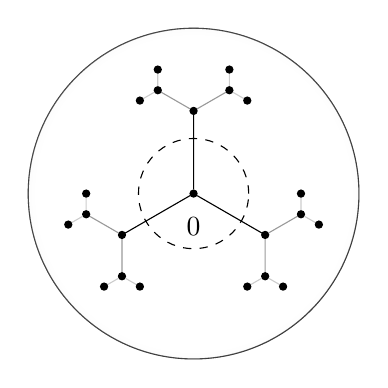
\begin{tikzpicture}[baseline=(current bounding box.center), scale=0.7]
% thanks to Tomasz M. Trzeciak
% based off of http://www.latex-community.org/viewtopic.php?f=4&t=2111

\draw (0,0) circle (3);

\begin{scope}
\pgfsetfading{fading3}{\pgftransformshift{\pgfpoint{0cm}{0cm}}}
\filldraw[black!5] (0,0) circle (3);
\end{scope}

\draw[dashed] (0,0) circle (1);
\coordinate[style={inner sep=0pt, outer sep=0pt, minimum size=3pt, fill=black, circle}] (O) at (0,0);
\node[below=5pt] at (O) {$0$};

\draw (O) -- +( 90:1.5) coordinate[style={inner sep=0pt, outer sep=0pt, minimum size=3pt, fill=black, circle}] (Q1)
      (O) -- +(210:1.5) coordinate[style={inner sep=0pt,outer sep=0pt,minimum size=3pt, fill=black,circle}] (Q2)
      (O) -- +(330:1.5) coordinate[style={inner sep=0pt,outer sep=0pt,minimum size=3pt, fill=black,circle}] (Q3);

\draw[black!40] (Q1) -- +(120-90:0.75) coordinate[style={inner sep=0pt, outer sep=0pt, minimum size=3pt, fill=black, circle}] (Q12)
      (Q1) -- +(240-90:0.75) coordinate[style={inner sep=0pt, outer sep=0pt, minimum size=3pt, fill=black, circle}] (Q13)
      (Q2) -- +(120-330:0.75) coordinate[style={inner sep=0pt, outer sep=0pt, minimum size=3pt, fill=black, circle}] (Q21)
      (Q2) -- +(240-330:0.75) coordinate[style={inner sep=0pt, outer sep=0pt, minimum size=3pt, fill=black, circle}] (Q23)
      (Q3) -- +(120-210:0.75) coordinate[style={inner sep=0pt, outer sep=0pt, minimum size=3pt, fill=black, circle}] (Q31)
      (Q3) -- +(240-210:0.75) coordinate[style={inner sep=0pt, outer sep=0pt, minimum size=3pt, fill=black, circle}] (Q32);

\draw[black!20] (Q12) -- +(90:0.375) coordinate[style={inner sep=0pt, outer sep=0pt, minimum size=3pt, fill=black, circle}] (Q121)
      (Q12) -- +(330:0.375) coordinate[style={inner sep=0pt, outer sep=0pt, minimum size=3pt, fill=black, circle}] (Q123)
      (Q13) -- +(90:0.375) coordinate[style={inner sep=0pt, outer sep=0pt, minimum size=3pt, fill=black, circle}] (Q131)
      (Q13) -- +(210:0.375) coordinate[style={inner sep=0pt, outer sep=0pt, minimum size=3pt, fill=black, circle}] (Q132)
      (Q21) -- +(90:0.375) coordinate[style={inner sep=0pt, outer sep=0pt, minimum size=3pt, fill=black, circle}] (Q212)
      (Q21) -- +(210:0.375) coordinate[style={inner sep=0pt, outer sep=0pt, minimum size=3pt, fill=black, circle}] (Q213)
      (Q23) -- +(210:0.375) coordinate[style={inner sep=0pt, outer sep=0pt, minimum size=3pt, fill=black, circle}] (Q231)
      (Q23) -- +(330:0.375) coordinate[style={inner sep=0pt, outer sep=0pt, minimum size=3pt, fill=black, circle}] (Q232)
      (Q31) -- +(210:0.375) coordinate[style={inner sep=0pt, outer sep=0pt, minimum size=3pt, fill=black, circle}] (Q312)
      (Q31) -- +(330:0.375) coordinate[style={inner sep=0pt, outer sep=0pt, minimum size=3pt, fill=black, circle}] (Q313)
      (Q32) -- +(90:0.375) coordinate[style={inner sep=0pt, outer sep=0pt, minimum size=3pt, fill=black, circle}] (Q321)
      (Q32) -- +(330:0.375) coordinate[style={inner sep=0pt, outer sep=0pt, minimum size=3pt, fill=black, circle}] (Q323);
\end{tikzpicture}%
%
\quad $\xrightarrow{\pi_{GH}}$ \quad%
%
\begin{tikzpicture}[baseline=(current bounding box.center), scale=0.8]

\newcommand\pgfmathsinandcos[3]{%
  \pgfmathsetmacro#1{sin(#3)}%
  \pgfmathsetmacro#2{cos(#3)}%
}
\newcommand\LongitudePlane[3][current plane]{%
  \pgfmathsinandcos\sinEl\cosEl{#2} % elevation
  \pgfmathsinandcos\sint\cost{#3} % azimuth
  \tikzset{#1/.style={cm={\cost,\sint*\sinEl,0,\cosEl,(0,0)}}}
}
\newcommand\DrawLongitudeCircle[2][1]{
  \LongitudePlane{35}{#2} % first argument is angle of elevation
  \tikzset{current plane/.prefix style={scale=#1}}
   % angle of "visibility"
  \pgfmathsetmacro\angVis{atan(sin(#2)*cos(35)/sin(35))} % these are angle of elevation too
  % this might assume that the angle of elevation is positive
  \draw[current plane] (\angVis:1) arc (\angVis:90:1);
  \draw[current plane,dashed] (\angVis:1) arc (\angVis:-90:1);
}

% the "2.5" magic number is the radius of the sphere 
% the "35" magic number is the angle of elevation of the camera
\pgfmathsetmacro\H{2.5*cos(35)}
\filldraw[ball color=white] (0,0) circle (2.5);
\foreach \t in {-5,-125,-245} { \DrawLongitudeCircle[2.5]{\t} }
\coordinate[style={inner sep=0pt,outer sep=0pt,minimum size=3pt,
    fill=black,circle}] (O) at (0,-\H);
\node[below=16pt] at (O) {$0$};
\coordinate[style={inner sep=0pt,outer sep=0pt,minimum size=3pt,
    fill=black,circle}] (I) at (0,\H);
\node[above=16pt] at (I) {$\infty$};
\end{tikzpicture}
\end{center}
\caption{The period map at $n = 2$, $p = 2$}\label{PeriodMapFigure}
\end{figure}

\begin{remark}
It is also possible to build versions of Dieudonn\'e theory over still more exotic rings.  The most successful such version is Zink's theory of \index{Dieudonn\'e module!display}Dieudonn\'e displays~\cite{ZinkDisplays}, which has found some application in algebraic topology~\cite{LawsonDisplays}.
\end{remark}









\section{Ordinary cooperations for Landweber flat theories}\label{LEFTCooperations}

\begin{center}
\textbf{Convention: We will write $H$ for $\HFp$ for the duration of the lecture.}
\end{center}

Our goal in this Lecture is to put Dieudonn\'e modules to work for us in algebraic topology.  The executive summary of Dieudonn\'e theory is that it gives a \emph{linear} presentation of the theory of Hopf algebras.  From the perspective of algebraic topology, functors sending cofiber sequences to exact sequences in a linear category are precisely the homology functors.  Tying these two ideas together, if we can find a functor that sends exact sequences of spaces (or spectra) to exact sequences of Hopf algebras, we can post-compose it with a suitable version of the Dieudonn\'e functor to get a homology functor and hence a \emph{spectrum}.

To meet algebraic topology in its natural setting, it will be useful to also have a version of Dieudonn\'e theory that is well-adapted to working with formal groups whose coordinate ring forms a \emph{graded} Hopf algebra.  Using as inspiration our previous identification
\begin{align*}
C(\G) & = \CatOf{FormalSchemes}(\A^1, \G) \\
& \cong \CatOf{FormalGroups}(\G, \widehat{C\W}_p) \\
& \cong \CatOf{HopfAlgebras}(\sheaf O_{\widehat{C\W}_p}, \sheaf O_{\G}),
\end{align*}
we are thus moved to form graded versions of the \index{Witt vectors!Hopf algebra}Witt Hopf algebra.  More precisely, the following theorem says that there are graded versions of the Witt Hopf algebra that give a sequence of projective generators for the category of connected graded Hopf algebras over $\F_p$:

\begin{theorem}[{\cite[Section 3.2]{Schoeller}, \cite[Proposition 1.6]{GLM}}]
Let $S(n)$ denote the free graded-commutative Hopf algebra over $\F_p$ on a single generator in degree $n > 0$.  There is a projective cover $H(n) \onto S(n)$, given by the formula
\begin{itemize}
\item If either of the following conditions hold...
\begin{itemize}
\item $p = 2$ and $n = 2^m k$ for $2 \nmid k$ and $m > 0$, \emph{or}
\item $p \ne 2$ and $n = 2p^m k$ for $p \nmid k$ and $m > 0$,
\end{itemize}
then $H(n) = \F_p[x_0, x_1, \ldots, x_k]$ with the Witt vector diagonal, i.e., the diagonal is arranged so that the elements $w_j = x_0^{p^j} + p x_1^{p^{j-1}} + \cdots + x_j$ are primitive.
\item Otherwise, $H(n) = S(n)$ is the identity.
\qed
\end{itemize}
\end{theorem}

\begin{corollary}
The category $\CatOf{GradedHopfAlgebras}^{> 0, \fin}_{\F_p/}$ of finite-type graded connected Hopf $\F_p$--algebras is a full subcategory of modules over \[\bigoplus_{n, m} \CatOf{GradedHopfAlgebras}(H(n), H(m)).\]
\end{corollary}
\begin{proof}[Proof sketch]
This is a general nonsense consequence of having found a set of projective generators.  The functor presenting the inclusion is \[M \mapsto \bigoplus_{n=0}^\infty \CatOf{GradedHopfAlgebras}(H(n), M),\] and since this functor is corepresented its automorphisms are encoded by the indicated ring.
\end{proof}

We would also like to give a set of conditions, analogous to the technical conditions appearing in the previous two presentations, which select this full subcategory out from all possible modules over this endomorphism ring.

\begin{definition}[{\cite[pg.\ 116]{GLM}}]
\index{Dieudonn\'e module!graded}Let $\CatOf{GradedDMods}$ denote the category of graded abelian groups $M$ equipped with maps\footnote{Here $n$ is required to be even if $p \ne 2$.}
\begin{align*}
V\co M_{pn} & \to M_n, &
F\co M_n & \to M_{pn}
\end{align*}
satisfying
\begin{enumerate}
\item $M_{< 1} = 0$.
\item If $n$ is odd, then $pM_n = 0$.
\item The composites are controlled by $FV = p$ and $VF = p$.\footnote{These come from the inclusion $H(n) \subseteq H(pn)$ and the map $H(pn) \to H(n)$ sending $x_n$ to $x_{n-1}^p$.}
\end{enumerate}
\end{definition}

\begin{remark}
Suppose that $n$ is even, written at odd primes in the form $n = 2p^m k$ with $p \nmid k$ or at $p = 2$ in the form $n = 2^m k$ with $2 \nmid k$ at $p = 2$.  Then, combining the above relations, we get the torsion condition $p^{m+1} M_n = F^{m+1} V^{m+1} M_n = 0$.
\end{remark}

\begin{theorem}[{\cite[Section 5]{Schoeller}, \cite[Theorem 1.11]{GLM}}]
The functor
\begin{align*}
D_*\co \CatOf{GradedHopfAlgebras}^{>0, \fin}_{\F_p/} & \to \CatOf{GradedDMods}, \\
D_*(H) = \bigoplus_n D_n(H) & = \bigoplus_n \CatOf{GradedHopfAlgebras}^{>0, \fin}_{\F_p/}(H(n), H)
\end{align*}
is an exact equivalence of categories.  Moreover, $D_* H(n)$ is characterized by the equation
\[\pushQED{\qed}
\CatOf{GradedDMods}(D_* H(n), M) = M_n. \qedhere
\popQED\]
\end{theorem}

Having produced our desired graded Dieudonn\'e theory, we now need some topological input.  We are by now well aware that the homology of an $H$--space forms a Hopf algebra, and the Serre spectral sequence for a fibration of $H$--spaces $F \to E \to B$ takes the form \[E_2^{*, *} = H^* B \otimes H^* F \Rightarrow H^* E.\]  The following result of Goerss--Lannes--Morel says that in the case that the fibration is one of \emph{infinite loopspaces}, we have the exactness property we need:

\begin{theorem}[{\cite[Lemma 2.8]{GLM}}]
Let $X \to Y \to Z$ be a cofiber sequence of spectra.  Then, provided $n > 1$ satisfies $n \not\equiv \pm 1 \pmod{2p}$, there is an exact sequence
\[\pushQED{\qed}
D_n H_* \Loops^\infty X \to D_n H_* \Loops^\infty Y \to D_n H_* \Loops^\infty Z. \qedhere
\popQED\]
\end{theorem}

\noindent This Theorem is not especially easy to prove: one works very directly with unstable modules over the Steenrod algebra, the bar spectral sequence, and Postnikov decomposition of infinite loopspaces.  We refer the reader to the paper directly, as we have been unable to find a useful improvement upon or even summary of the results presented there.  Nonetheless, granting this Theorem, we use Brown representability to draw the following consequence:

\begin{corollary}[{\cite[Theorem 2.1, Remark 2.9]{GLM}}]\label{BrownGitlerSpectraDefn}
For $n > 1$ an integer satisfying $n \not\equiv \pm 1 \pmod{2p}$,\footnote{As convention, when $n \equiv \pm 1 \pmod{2p}$ we set $B(n) := B(n-1)$, and $B(0) := \S^0$.} the \index{Brown--Gitler spectrum}\textit{Brown--Gitler spectrum} $B(n)$ is the spectrum satisfying \[\pushQED{\qed}B(n)_n X \cong D_n H_* \Loops^\infty X. \qedhere\popQED\]
\end{corollary}

Before exploiting this result to compute something about unstable cooperations, we will prove a sequence of small results making these spectra somewhat more tangible.

\begin{lemma}[{\cite[Lemma 3.2]{GLM}}]
The spectrum $B(n)$ is connective and $p$--complete.
\end{lemma}
\begin{proof}
First, rearrange:
\begin{align*}
\pi_k B(n) & = B(n)_n \S^{n-k} = D_n H_* \Loops^\infty \Susp^\infty S^{n-k}.
\end{align*}
If $k < 0$, $n$ is below the connectivity of $\Loops^\infty \S^{n-k}$ and hence this vanishes.  The second assertion follows from the observation that $H\Z_* B(n)$ is an $\F_p$--module, followed by an Adams spectral sequence argument.  To see the assertion about being an $\F_p$--module, restrict to the case $n \not\equiv \pm 1 \pmod{2p}$ and calculate
\begin{align*}
H\Z_k B(n) & = B(n)_n \Susp^{n-k} H\Z \\
& = D_n H_* K(\Z, n-k) \\
& = [H(n), H_* K(\Z, n-k)]_n \\
& = [Q^* H_* K(\Z, n-k)]_n. \qedhere
\end{align*}
\end{proof}

We can use a similar trick as in the second part of the proof to calculate the cohomology groups $H^* B(n)$:

\begin{definition}[{\cite[Example 3.6]{GLM}}]\label{SpanierWhiteheadDualOfGeneratingModule}
Let $G(n)$ be the free \index{Steenrod algebra!unstable module}unstable $\mathcal A^*$--module on one generator of degree $n$, so that if $M$ is an unstable $\mathcal A^*$--module then \[\CatOf{Modules}_{\mathcal A^*}(G(n), M) = M_n.\]  This module admits a presentation as \[G(n) = \begin{cases} \Susp^n \mathcal A / \{\beta^\eps P^i \mid 2pi + 2\eps > n\}\mathcal A & \text{if $p > 2$}, \\ \Susp^n \mathcal A / \{\Sq^i \mid 2i > n\}\mathcal A & \text{if $p = 2$}. \end{cases}\]  The Spanier--Whitehead dual of this right-module, $DG(n)$, is given by \[\Susp^n (D G(n))^* = \begin{cases}\mathcal A / \mathcal A \{\chi(\beta^\eps P^i) \mid 2pi + 2\eps > n\} & \text{if $p > 2$}, \\ \mathcal A / \mathcal A \{\chi{\Sq^i} \mid 2i > n\} & \text{if $p = 2$}. \end{cases}\]
\end{definition}

\begin{theorem}[{\cite[Proof of Theorem 3.1]{GLM}}]
There is an isomorphism \[H^* B(n) \cong \Susp^n(DG(n))^*.\]
\end{theorem}
\begin{proof}
We restrict attention to $n \not\equiv \pm 1 \pmod p$, where we can use \Cref{BrownGitlerSpectraDefn} directly.  Start, as before, by addressing the dual problem of computing the mod--$p$ homology:
\begin{align*}
H_k B(n) = B(n)_n \Susp^{n-k} H = D_n H_* K(\F_p, n-k).
\end{align*}
The unstable module $G(n)$ also enjoys a universal property in the category of \emph{stable} $\mathcal A^*$--modules, by passing to the maximal unstable quotient $\Loops^\infty M$ of a stable module $M$: \[\CatOf{Modules}_{\mathcal A^*}(G(n), M) \cong [\Loops^\infty M]_n.\]  Hence, we can continue our computation:
\begin{align*}
H_k B(n) & = D_n H_* K(\F_p, n-k) \\
& = \CatOf{Modules}_{\mathcal A^*}(G(n), \Susp^{n-k} \mathcal A_*) \\
& = \CatOf{Modules}_{\F_p}(G(n)_{n-k}, \F_p).
\end{align*}

We learn immediately that $H_* B(n)$ is finite.  We would like to show, furthermore, that $H_* B(n)$ is the Spanier--Whitehead dual $\Susp^n DG(n)$.  It suffices to show \[\CatOf{Modules}_{\mathcal A^*}(G(n), \Susp^j \mathcal A_*) = \CatOf{Modules}_{\mathcal A^*}(\F_p, \Susp^j \mathcal A_* \otimes H_* B(n))\] for all values of $j$.  This follows from calculating $B(n)_n \Susp^{n+j} H$ using the same method.  Finally, we apply linear-algebraic duality and \Cref{SpanierWhiteheadDualOfGeneratingModule}.
\end{proof}

Lastly, for a \emph{space} $X$, we definitionally have that have $H_* X$ forms an unstable module over the Steenrod algebra, i.e., $\Loops^\infty H_* X = H_* X$.  This has the following direct sequence (with minor fuss at the bad indices $n \equiv \pm 1 \pmod p$):

\begin{lemma}[{\cite[Lemma 3.3]{GLM}}]
For $X$ a space, there is a natural surjection
\[\pushQED{\qed}
B(n)_n X \to H_n X. \qedhere
\popQED\]
\end{lemma}



Let's now work toward using the $B(n)$ spectra to analyze the \index{Hopf ring}Hopf rings arising from unstable cooperations.  Our intention is to prove the following:
\begin{theorem}[{cf.\ \Cref{UnstableEthyCooperations}}]\label{LEFTUnstableCooperations}
For $F = H$ and $E$ a \index{Landweber flat}Landweber flat homology theory, the comparison map \[\AA(H, E) \to H_* \OS{E}{2*}\] is an isomorphism of Hopf rings.
\end{theorem}
\noindent We have previously computed that the comparison map \[\AA(H, BP) \to H_* \OS{BP}{2*}\] is an isomorphism.  We will now reimagine this statement in terms of Dieudonn\'e theory, but in order to do this we first have to reimagine some of Dieudonn\'e theory itself, as our description of it is concerned with \emph{Hopf algebras} rather than \emph{Hopf rings}.  A Hopf ring is not much structure on top of an (externally) graded system of (internally) graded Hopf algebras $A_*$: it is a multiplication map \[\circ\co A_* \boxtimes A_* \to A_*,\] where ``$\boxtimes$'' is a kind of graded \index{Hopf algebra!tensor product}tensor product of externally graded Hopf algebras~\cite[Proposition 2.6]{HuntonTurner}, \cite[Definition 2.2]{BuchstaberLazarev}, \cite[Section 5]{GoerssDieudonne}.  Since $D_*$ gives an equivalence of categories between internally graded Hopf algebras and internally graded Dieudonn\'e modules, we should be able to find an analogous formula for the tensor product of \index{Dieudonn\'e module!tensor product}Dieudonn\'e modules.

\begin{definition}{\cite[pg.\ 154]{GoerssDieudonne}}
The naive tensor product $M \otimes N$ of Dieudonn\'e modules $M$ and $N$ receives the structure of a $\W(k)[V]$--module, where $V(x \otimes y) = V(x) \otimes V(y)$.  We define the \textit{tensor product of Dieudonn\'e modules}\footnote{This definition is specialized to $\F_p$, where we don't have to worry about Frobenius semi-linearity.} by \[M \boxtimes N = \left.\frac{\W(k)[F, V]}{(VF = p)} \otimes_{\W(k)[V]} (M \otimes N) \middle/ \left( \begin{array}{c} 1 \otimes Fx \otimes y = F \otimes x \otimes Vy, \\ 1 \otimes x \otimes Fy = F \otimes Vx \otimes y \end{array} \right) \right. .\]
\end{definition}

\begin{lemma}[{\cite[Corollary 8.14]{GoerssDieudonne}}]
The natural map \[D_*(M) \boxtimes D_*(N) \to D_*(M \boxtimes N)\] is an isomorphism. \qed
\end{lemma}

\begin{definition}
For a ring $R$, a \index{Dieudonn\'e module!algebra}\textit{Dieudonn\'e $R$--algebra} $A_*$ is an externally graded Dieudonn\'e module equipped with an $R$--action and a unital multiplication \[\circ\co A_* \boxtimes A_* \to A_*.\]
\end{definition}

\begin{example}[{\cite[Proposition 10.2]{GoerssDieudonne}}]
Inspired by \Cref{UnstableRWRelation} and our interest in $H_* \OS{E}{*}$, for a complex-oriented homology theory $E$ we define its \textit{algebraic Dieudonn\'e $E_*$--algebra} by \[R_E = \left. E_*[b_1, b_2, \ldots] \middle/ \left( \begin{array}{c} b(s+t) = b(s) +_E b(t) \end{array} \right) \right.,\] where $V$ is multiplicative, $V$ fixes $E_*$, and $V$ satisfies $Vb_{pj} = b_j$.\footnote{If $E_*$ is torsion-free, then this determines the behavior of $F$ by $FV = p$.}  We also write $D_E = \{D_{2m} H_* \OS{E}{2n}\}$ for the even part of the topological Dieudonn\'e algebra, and these come with natural comparison maps \[R_E \to D_E \to D_* H_* \OS{E}{2*}.\]
\end{example}

\begin{theorem}[{\cite[Theorem 11.7]{GoerssDieudonne}}]\label{LandweberFlatUnstableCoopns}
Restricting attention to the even parts, the maps \[R_E \to D_E \to D_* H_* \OS{E}{2*}\] are isomorphisms for $E$ Landweber flat.
\end{theorem}
\begin{proof}
In \Cref{HopfRingForEBP}, we showed that these maps are isomorphisms for $E = BP$.  However, the right--hand object can be identified via Brown--Gitler juggling: \[D_n H_* \OS{E}{2j} = B(n)_n \Susp^{2j} E = E_{2j+n} B(n).\]  It follows that if $E$ is Landweber flat, then the middle-- and right--terms are determined by change-of-base from the respective $BP$ terms.  Finally, the left term commutes with change-of-base by its algebraic definition, and the theorem follows.
\end{proof}

\begin{remark}
Goerss's original proof of \Cref{LandweberFlatUnstableCoopns}~\cite{GoerssDieudonne} involved a lot more work, essentially because he didn't want to assume \Cref{HFpBPCooperationsTheorem} or \Cref{HopfRingForEBP}.  Instead, he used the fact that $\Susp^\infty_+ \Loops^2 S^3$ is a regrading of the ring spectrum $\bigvee_n B(n)$, together with knowledge of $BP_* \Loops^2 S^3$.  Since we have already done the hard work of proving \Cref{HFpBPCooperationsTheorem}, we are not obligated to pursue this other line of thought.
\end{remark}

\begin{remark}[{\cite[Proposition 11.6, Remark 11.4]{GoerssDieudonne}}]
The Dieudonn\'e algebra framework also makes it easy to add in the odd part after the fact.  Namely, suppose that $E$ is a torsion--free ring spectrum and suppose that $E_* B(n)$ is even for all $n$.  In this setting, we can verify the purely topological version of this statement: \index{homology suspension}the map \[D_E[e] / (e^2 - b_1) \to D_* H_* \OS{E}{*}\] is an isomorphism.  To see this, note that because \[E_{2n-2k-1} B(2n) \to D_{2n} H_* \OS{E}{2k+1}\] is onto and $E_{2n-2k-1} B(2n)$ is assumed zero, the group $D_{2n} H_* \OS{E}{2k+1}$ vanishes as well.  A bar spectral sequence argument shows that $D_{2n+1} H_* \OS{E}{2k+2}$ is also empty~\cite[Lemma 11.5.1]{GoerssDieudonne}.  Hence, the map on even parts \[(D_E[e] / (e^2 - b_1))_{*, 2n} \to (D_* H_* \OS{E}{*})_{*, 2n}\] is an isomorphism, and we need only show that \[D_* H_* \OS{E}{2n} \xrightarrow{e \circ -} D_* H_* \OS{E}{2n+1}\] is an isomorphism as well.  Since we have $e(Fx) = F(Ve \circ x) = 0$ generally and $D_* A / FD_* A \cong Q^* A$ for a Hopf algebra $A$, we see that $e$ kills decomposables and suspends indecomposables: \[e \circ D_* H_* \OS{E}{2n} = \Susp QH_* \OS{E}{2n}.\]  This is also what happens in the bar spectral sequence, and the claim follows.  In light of \Cref{LandweberFlatUnstableCoopns}, this means that for Landweber flat $E$, the comparison isomorphism can be augmented to a further isomorphism \[R_E[e] / (e^2 - b_1) \to D_* H_* \OS{E}{*}.\]
\end{remark}

\begin{remark}[{\cite{HopkinsHunton}}]
The results of this Lecture are accessed from a different perspective by Hopkins and Hunton, essentially by forming a tensor product of Hopf rings and showing that Landweber flatness induces a kind of flatness with respect to the Hopf ring tensor product as well.
\end{remark}










\section{Cooperations among geometric points on \texorpdfstring{$\moduli{fg}$}{Mfg}}\label{CoopnsForMoravaKandHA}


Our discussion of unstable cooperations has touched on each of the families of chromatic homology theories described in \Cref{DefnChromaticHomologyThys} except one: the \index{Morava K theory@Morava $K$--theory}\index{Morava E theory@Morava $E$--theory}Morava $K$-- and $E$--theories.  Our final goal before moving on to other subjects is to describe some of the \index{operations!mixed}\index{operations!unstable}mixed unstable cooperations for $(K_\Gamma)_* \OS{K_{\Gamma'}}{*}$.  In complete generality, this seems like a difficult problem: our algebraic model is rooted in formal group homomorphisms, and we have not proven any theorems about the moduli of such for arbitrary finite-height formal groups.  However, the landscape brightens considerably in the case where we pick $\Gamma' = \G_a$, as this is the sort of calculation we considered in \Cref{LazarevComparisonOfCplxes} and \Cref{CalculationOfLTTangentSpace}.  In light of this, we specialize $\Gamma'$ to $\G_a$ (and hence $K_{\Gamma'}$ to an Eilenberg--Mac Lane spectrum $H$), and we abbreviate $K_\Gamma$ to just $K$.

As with all the other major results of this Case Study, our approach will rest on the \index{bar spectral sequence}bar spectral sequence \[\Tor^{K_* \OS{H}{q}}_{*, *}(K_*, K_*) \Rightarrow K_* \OS{H}{q+1}.\]  The analysis of this spectral sequence was first accomplished by Ravenel and Wilson~\cite{RavenelWilsonKthyOfEMSpaces}, but has since been re-envisioned by Hopkins and Lurie~\cite[Section 2]{HopkinsLurie}.  In order to give an effective analysis of this spectral sequence in line with the theme of this book, we will endeavor to give algebro-geometric interpretations of its input and its output, beginning with the case $q = 0$ and $H = H(S^1[p^j])$ for some $1 \le j \le \infty$.  This task itself begins with giving just \emph{algebraic} descriptions of the input and output.  For $j < \infty$, we have essentially already computed the output by other means:

\begin{theorem}[{\cite[Theorem 5.7]{RavenelWilsonKthyOfEMSpaces}, \cite[Proposition 2.4.4]{HopkinsLurie}}]\label{KtheoryConvertsTorsionToTorsion}
There is an isomorphism \[BS^1[p^j]_K \cong BS^1_K[p^j].\]
\end{theorem}
\begin{proof}[Remarks on proof]
In \Cref{MUConvertsTorsionPointsToTorsionPoints}, we have already shown a very similar statement.  The crux of that argument was to show that multiplication by the $p$--series in $MU^* \CP^\infty$ was injective without knowing very much about the ground ring $MU^*$.  Here our task is even easier: any \index{formal group!l series@$\ell$--series}$p$--series for $\Gamma$ takes the form $[p](x) = c x^{p^d} + \cdots$ for $c$ a unit.  Such an element is certainly not a zero-divisor.
\end{proof}

\begin{remark}\label{KHomologyOfClassifyingSpace}
In the proof of the homological statement dual to \Cref{KtheoryConvertsTorsionToTorsion}, there is a corresponding exact sequence of Hopf algebras
\begin{center}
\begin{tikzcd}
& K_* BS^1 \arrow{rd}{- \frown [p^j](x)} \\
K_*(BS^1[p^j]) \arrow{ru} & & K_* BS^1, \arrow{ll}{\partial}
\end{tikzcd}
\end{center}
where again $\partial = 0$ and hence $K_*(BS^1[p^j])$ is presented as the kernel of the map ``cap with $[p^j](x)$''.  We will revisit this duality in the next Case Study.
\end{remark}

With this in hand, the analysis of the bar spectral sequence proceeds very much analogously to the example of the unstable dual Steenrod algebra of \Cref{UnstableContextsSection}.  We will analyze what \emph{must} happen in the bar spectral sequence \[\Tor^{K_* S^1[p^j]}_{*, *}(K_*, K_*) \Rightarrow K_* BS^1[p^j]\] in order to reach the conclusion of \Cref{KtheoryConvertsTorsionToTorsion}.  In the input to this spectral sequence, the ground algebra is given by a noncanonical isomorphism \[K_* \OS{H(S^1[p^j])}{0} \cong K_* \OS{H\Z/p^j}{0} = K_*[[1]] / ([1]^{p^j} - 1) = K_*[[1] - [0]] / \<[1] - [0]\>^{p^j}.\]  The $\Tor$--algebra for this truncated polynomial algebra $K_*[a_\emptyset] / a_\emptyset^{p}$ is then given by the formula \[\Tor^{K_*[a_\emptyset] / a_\emptyset^{p^j}}_{*, *}(K_*, K_*) = \Lambda[a'_\emptyset] \otimes \Gamma[a_\emptyset],\] the combination of an exterior algebra and a divided power algebra.\footnote{In Ravenel--Wilson~\cite[Lemma 6.6]{RavenelWilsonKthyOfEMSpaces}, the elements $a_\emptyset$ and $a'_\emptyset$ are identified as a \idxentry{transpotence} and a \idxentry{homology suspension} respectively.}  We know which classes are supposed to survive this spectral sequence, and hence we know where the differentials must be:
\begin{align*}
d(a_\emptyset)^{[p^{jd}]} & = a'_\emptyset, \\
\Rightarrow d(a_\emptyset)^{[i + p^{jd}]} & = a'_\emptyset \cdot a_\emptyset^{[i]}.
\end{align*}
The spectral sequence collapses after this differential.  In the case $1 < j < \infty$, there are some hidden multiplicative extensions in the spectral sequence, but these too are all determined by already knowing the multiplicative structure on $K_* \OS{H(S^1[p^j])}{1}$.

However, the case of $j = \infty$ is a bit different, beginning with the following Lemma:

\begin{lemma}
For $q \ge 1$, there is a $p$--adic equivalence of $K(\Q/\Z_{(p)}, q)$ with $K(\Z, q+1)$.
\end{lemma}
\begin{proof}
This is a consequence of the fiber sequence \[K(\Q, q) \to K(\Q/\Z_{(p)}, q) \to K(\Z_{(p)}, q+1).\]  The first term has vanishing mod--$p$ homology, forcing the $\HFp$--Serre spectral sequence of the fibration to collapse and for the edge homomorphism to be an isomorphism.  Similarly, the map $K(\Z, q+1) \to K(\Z_{(p)}, q+1)$ is an equivalence on mod--$p$ homology.
\end{proof}

\begin{remark}
Thinking of $K(\Z, q+1)$ as $B^q S^1$, one can also think of this theorem as giving a $p$--adic equivalence between $B^q(S^1[p^\infty])$ and $B^q S^1$---i.e., the prime--to--$p$ parts of $S^1$ do not matter for $p$--adic homotopy theory.
\end{remark}

We use this to continue the analysis of the case $q = 1$ and $j = \infty$, where the Lemma gives $B(S^1[p^\infty]) = \CP^\infty$.  The bar spectral sequence of interest then takes the form \[\Tor^{K_* S^1}_{*, *}(K_*, K_*) \Rightarrow K_* \CP^\infty.\]  The input algebra $K_* S^1$ is exterior on a single generator in odd degree, and so its $\Tor$--algebra is linearly dual to a power series algebra on a single generator in even degree.  Since all of its input is even, this spectral sequence collapses immediately.

There is a lot of structure visible in this collection of spectral sequences, as considered simultaneously.  Without further inspection, the spectral sequence at $j = \infty$ records that $\CP^\infty_K$ is a formal variety, and the spectral sequences at the finite values $1 \le j < \infty$ encode in their differentials the behavior of the map $p^j\co \Gamma \to \Gamma$ on functions---indeed, this appears to be the entire job of $a'_\emptyset$.  Lastly, we notice that the $E_\infty$ page of each finite-range spectral sequence includes into the spectral sequence at $j = \infty$, and moreover this filtration is exhaustive: every term in the $j = \infty$ spectral sequence appears at some $j < \infty$ stage.  Since this last property is about the $E_\infty$ pages, it is really a property of the formal group $\Gamma$, which we record in a definition:

\begin{definition}[{\cite[Definition 4.1]{GrothendieckCristaux}}]
A \index{p divisible group@$p$--divisible group}\textit{$p$--divisible group}\footnote{Some like to call these \index{Barsotti--Tate group|see {$p$--divisible group}}\textit{Barsotti--Tate groups}, which is probably the better name, since ``$p$--divisible group'' sounds like a property rather than all this data.} over a field $k$ is a system $\mathbb G_j$ of finite group schemes and inclusions $i_k^j\co \mathbb G_k \to \mathbb G_j$ for $k < j$ which model the inclusions $\mathbb G_j[p^k] \subseteq \mathbb G_j$.
\end{definition}

\begin{definition}
A $p$--divisible group is said to be \index{p divisible group@$p$--divisible group!connected}\textit{connected} when its constituent subgroups $\mathbb G_j$ are infinitesimal thickenings of $\Spec k$.  An example of this is the sequence of torsion subgroups $\G[p^j]$ of a formal group $\G$.  A \emph{nonexample} of this is the sequence of constant group schemes $\G_j = S^1[p^j]$.
\end{definition}

\begin{lemma}[{\cite[Section 6.7]{GrothendieckCristaux}}]
Over a perfect field of positive characteristic $p$, a connected $p$--divisible group is equivalent to a smooth formal group of finite height.
\end{lemma}
\begin{proof}[Correspondence]
The maps in both directions are easy: a $p$--divisible group is sent to its colimit, and a formal group of finite height is sent to its system of $p^j$--torsion subgroups.  In both directions there is something mild to check: that the colimit gives a formal variety, and that the system of $p^j$--torsion subgroups has the indicated exactness properties.
\end{proof}

We will soon see that these interrelations among the bar spectral sequences for the different Eilenberg--Mac Lane spaces, as well as the special behavior of the spectral sequence at $j = \infty$, are generic phenomena in $q$.  We record the steps in our upcoming induction in the following Theorem:

\begin{theorem}[{\cite[Theorems 2.4.11--13]{HopkinsLurie}}]\label{MainKThyOfEMSpacesTheorem}
The following claims give a complete description of the Morava $K$--theory schemes associated to the Eilenberg--Mac Lane spaces $\OS{HS^1[p^j]}{q}$.
\begin{enumerate}
    \item The formal scheme $(\OS{H(S^1[p^\infty])}{q})_K$ is a formal variety of dimension $\binom{d-1}{q-1}$.
    \item Suppose that $(\OS{H(S^1[p^\infty])}{q-1})_K$ is a $p$--divisible formal group of height $\binom{d}{q-1}$ and dimension $\binom{d-1}{q-1}$, that $(\OS{H(S^1[p])}{q-1})_K$ models its $p$--torsion, and that the cup product induces an isomorphism \[\theta^{q-1}\co \Q / \Z_{(p)} \otimes D(\OS{H(S^1[p^\infty])}{1})^{\wedge (q-1)} \to D(\OS{H(S^1[p^\infty])}{q-1}),\] where $D(G)$ denotes the \index{Dieudonn\'e module}Dieudonn\'e module associated to $K_0(G)$, where \[K_*(G) = K_0(G) \otimes_k K_*\] is a $p$--divisible Hopf algebra.  The same claims are then true with $q-1$ replaced everywhere by $q$.
    \item Consider the model $\Q / \Z_{(p)} \cong S^1[p^\infty]$ for the $p$--primary part of the circle group.  Suppose that for each $j$, the short exact sequence of groups \[0 \to \frac{1/p^j \cdot \Z_{(p)}}{\Z_{(p)}} \to \frac{\Q}{\Z_{(p)}} \to \frac{\Q}{1/p^j \cdot \Z_{(p)}} \to 0\] induces a short exact sequence of group-schemes upon applying $(\OS{H(-)}{q-1})_K$.  The sequence of group schemes under $(\OS{H(-)}{q})_K$ is then also short-exact.
\end{enumerate}
\end{theorem}
\begin{proof}[Proof of Part 1]\renewcommand{\qedsymbol}{\relax}
This claim turns out to be entirely algebraic and a matter of being able to compute $H^*(\mathbb G; \G_a)$ for $\mathbb G$ a connected $p$--divisible group.  This is expressed in the main algebraic result of Hopkins--Lurie:
\end{proof}

\begin{theorem}[{\cite[Theorem 2.2.10]{HopkinsLurie}}]
Let $\mathbb G$ be a $p$--divisible group over a perfect field $k$ of positive characteristic $p$.  There is then an isomorphism \[H^*(\mathbb G; \G_a) \cong \Sym^*(\Susp H^1(\mathbb G[p], \G_a)),\] where ``$\Susp$'' indicates that the classes are taken to lie in degree $2$. \qed
\end{theorem}

\begin{lemma}[{\cite[Remark 2.2.5]{HopkinsLurie}}]
If $\mathbb G$ is a connected $p$--divisible group of height $d$ and of dimension $n$ as a formal variety, then
\[\pushQED{\qed}
\operatorname{rank}\left(H^1(\mathbb G[p]; \G_a)\right) = d - n. \qedhere
\popQED\]
\end{lemma}

\begin{remark}
In the case where $\mathbb G = \Gamma$ is the original height $d$ formal group of dimension $1$, this computes $H^*(\Gamma; \G_a)$ to be a power series algebra on $(d-1)$ generators.  This is precisely the result we recorded by hand in \Cref{CalculationOfLTTangentSpace}.
\end{remark}

\noindent Returning to the task at hand, we assume inductively that $(\OS{H(S^1[p^\infty])}{q-1})_K$ is a connected $p$--divisible group of height $\binom{d}{q-1}$ and dimension $\binom{d-1}{q-1}$.  Since the input to the bar spectral sequence is computed by formal group cohomology (\cite{LazarevDeformations}, \cite[Example 2.3.5]{HopkinsLurie}, Proof of \Cref{Symmetric2CocycleLemma}), it follows that the instance computing $K^* \OS{H(S^1[p^\infty])}{q}$ has $E_2$--page an even-concentrated power series algebra of dimension \[\binom{d}{q-1} - \binom{d-1}{q-1} = \binom{d-1}{q}.\]  The spectral sequence therefore collapses at this page, so that $(\OS{H(S^1[p^\infty])}{q})_K$ is a formal variety of the dimension claimed.

\begin{proof}[Proof of Part 2, with a gap]\renewcommand{\qedsymbol}{\relax}
The other claims in Part 2 are formal after we check that $\theta^q$ is an isomorphism, since the $p$--power--torsion structure of \[(\OS{H(S^1[p^\infty])}{q})_K\] can be read off from its Dieudonn\'e module, as can its height.  We introduce notation to analyze this statement: set $M$ to be the Dieudonn\'e module associated to $K_* \CP^\infty$, i.e., \[M = D(\OS{H(S^1[p^\infty])}{1}).\]  In the following diagram
\begin{center}
\begin{tikzcd}
0 \arrow{r} & M^{\wedge q} \arrow{r} \arrow{d}{V} & \Q \otimes M^{\wedge q} \arrow{r} \arrow{d}{V} & \Q / \Z_{(p)} \otimes M^{\wedge q} \arrow{r} \arrow{d}{V} & 0 \\
0 \arrow{r} & M^{\wedge q} \arrow{r} & \Q \otimes M^{\wedge q} \arrow{r} & \Q / \Z_{(p)} \otimes M^{\wedge q} \arrow{r} & 0
\end{tikzcd}
\end{center}
the middle map is an isomorphism.  This forces $V$ to be a surjective endomorphism of $M^{\wedge q} \otimes \Q/\Z_{(p)}$, and the snake lemma shows that there is an isomorphism \[\ker(V\co \Q/\Z_{(p)} \otimes M^{\wedge q} \to \Q/\Z_{(p)} \otimes M^{\wedge q}) \cong \operatorname{coker}(V\co M^{\wedge q} \to M^{\wedge q}).\]  Picking any coordinate $x$ and considering it as an element in the curves model of the Dieudonn\'e functor, we see that the right-hand side is spanned by elements $x \sm V^{\sm I} x$, and hence the left-hand side has $k$--vector--space dimension $\binom{d-1}{q}$.

By very carefully studying the bar spectral sequence, one can learn that $\theta^q$ induces a surjection\footnote{The proof of this is quite complicated, and it rests on a pairing between the spectral sequence for $q = 1$ and the spectral sequence at $q - 1$, mapping to the spectral sequence for $q$.  Remarkably, this same pairing is the main tool that powers the original approach of  Ravenel--Wilson~\cite{RavenelWilsonKthyOfEMSpaces}.  There, their program is to fix $j = 1$ and inductively analyze $q$ using this same pairing, then use these base cases to ground a strong induction on $j$ and $q$, and then finally to fix $q$ and take the limit as $j \to \infty$.} \[\ker V|_{\Q / \Z_{(p)} \otimes M^{\wedge q}} \to \ker V|_{D(\OS{H(S^1[p^\infty])}{q})}.\]  In fact, since these two have the same rank, $\theta^q|_{\ker V}$ is an isomorphism on these subspaces.  This is enough to conclude that $\theta^q$ is an injection: since the action of $V$ is locally nilpotent, if $\theta^q$ ever failed to be an injection then we could apply $V$ enough times to get an example of a nontrivial element in $\ker V|_{\Q / \Z_{(p)} \otimes M^{\wedge q}}$ mapping to zero.  Finally, to show that $\theta^q$ is surjective, we again use the local nilpotence of $V$ to filter $\Q / \Z_{(p)} \otimes M^{\sm q}$ by the subspaces $\ker V^\ell$, $\ell \ge 1$, and it is then possible (though we admit the proof) to use our understanding of $\ker V$ to form preimages.
\end{proof}

\begin{proof}[Proof of Part 3, mostly omitted]
This proof is quite complicated, but it is, in spirit, a generalization of the observation at $q = 1$ that the role of the odd-degree classes in the bar spectral sequence is to pair up with those classes in the image of the $[p^j]$--map.  In fact, their main assertion is:
\begin{quote}
We give notation for the following rings:
\begin{align*}
A & = K_0 \OS{H(S^1[p^\infty])}{q-1}, &
A' & = K_0 \OS{H(S^1[p^j])}{q-1}, &
R & = K_0 \OS{H(S^1[p^\infty])}{q}.
\end{align*}
Let $x' \in E_2^{1, 0}$ be an element, and let $y' \in \mathfrak m_R$ satisfy \[y' = \psi(x') \otimes v \in \Ext^2_A \otimes_k \pi_2 K \cong \mathfrak m_R / \mathfrak m_R^2.\]  Suppose that the Hopf algebra homomorphism $[p^j]\co R \to R$ carries $y'$ to an element $y \in \mathfrak m_R^s$, and let $x \in E_2^{2s, 2s-2}$ denote the image of $y$ under the composite \[\mathfrak m_R^s / \mathfrak m_R^{s+1} \cong \Ext_A^{2s} \otimes_k \pi_{2s} K \to \Ext_{A'}^{2s} \otimes_k \pi_{2s} K = E_2^{2s, 2s} \xrightarrow{-v^{-1}} E_2^{2s, 2s-2}.\]  Then $x$ and $x'$ survive to the $(2s - 1)${\th} page of the bar spectral sequence, and there we have \[d_{2s-1} x' = x.\]
\end{quote}
From here, it is a matter of \emph{very} carefully pairing elements up (cf.\ \cite[pg.\ 60]{HopkinsLurie}).
\end{proof}

\begin{remark}
\Cref{MainKThyOfEMSpacesTheorem} admits a restatement purely in terms of \index{Hopf algebra}Hopf algebras, although Dieudonn\'e theory was essential in its proof.  The cup product gives a natural map \[\Alt^q K_* \OS{H(S^1[p^j])}{1} \to K_* \OS{H(S^1[p^j])}{q},\] where ``$\Alt$'' refers to the alternating \index{Hopf algebra!alternating}Hopf algebra.\footnote{Note that this alternation condition becomes dramatically more complicated in the case that the formal group law and its formal group inverse series become more complicated than that of $\G_a$.}  The main result of this section is that this map is an isomorphism for all $q$, and indeed that the map from the free alternating Hopf \emph{ring} maps isomorphically to the topological Hopf ring.
\end{remark}

\begin{remark}[{\cite[Section 3]{HopkinsLurie}, \cite{HedayatzadehGeneralCase}, \cite{HedayatzadehFieldCase}}]\label{EThyOfEMSpaces}
\todo{Mention Ravenel--Wilson--Yagita's work, especially the difference between cohomology and homology, and matters of continuous $E$--theory.}
Because $K^* \OS{H\Z/p^j}{q}$ is even, you can hope to augment this to a calculation of $E^* \OS{H\Z/p^j}{q}$ for $E = E_\Gamma$ the associated Morava $E$--theory.  This is indeed possible, and the analogous formula is true at the level of Hopf algebras: \[E_* \OS{H(S^1[p^j])}{q} \cong \Alt^q E_* \OS{H(S^1[p^j])}{1}.\] However, the attendant algebraic geometry is quite complicated: you either need a form of Dieudonn\'e theory that functions over $\context{E_\Gamma}$ (and then attempt to drag the proof above through that setting), or you need to directly confront what ``\index{p divisible group@$p$--divisible group!alternating power}alternating power of a $p$--divisible group'' means at the level of $p$--divisible groups (and forego all of the time-saving help afforded to you by Dieudonn\'e theory).
\end{remark}

\begin{remark}[{cf.\ \Cref{StableMixedKthyCoopnsVanish}}]
You'll notice that in $K_* \OS{H}{q+1}$ if we let the $q$--index tend to $\infty$, we get the $K$--homology of a point.  This is another way to see that the stable cooperations $K_* H$ vanish, meaning that the \emph{only} information present comes from unstable cooperations.
\end{remark}

\begin{remark}
Although the method of starting with the $j = \infty$ case and deducing from it the $1 \le j < \infty$ cases is due to Hopkins and Lurie, the observation that the spectral sequence at $j = \infty$ is remarkably simple had already been made by Ravenel and Wilson~\cite[Theorem 12.3]{RavenelWilsonKthyOfEMSpaces},~\cite[Theorem 8.1.3]{RWY}.
\end{remark}

\begin{remark}
\Cref{MainKThyOfEMSpacesTheorem} has a statement in the language of \Cref{UnstableAlgebraicModelSection}.  Rather than forming the algebraic approximation \[\AA(K, H) = K_*(\CP^\infty)_{K_*[H_*]}^{\circulatearrows}[H_* \CP^\infty]\] as usual, we form the modified version \[\AA_{p^j}(K, H) = K_*(\OS{H(S^1[p^j])}{1})_{K_*[H_*]}^{\circulatearrows}[H_* \OS{H(S^1[p^j])}{1}].\]  Using the same unstable Kronecker pairing, this supports a natural map to $K_* \OS{H}{*}$, and a summary of this Lecture's results is that it is an isomorphism.  In particular, this auxiliary approximation makes use of \emph{odd}--dimensional Eilenberg--Mac Lane spaces.
\end{remark}











